\documentclass[11pt]{article}
\usepackage{amsmath}
\usepackage{amsfonts}
\usepackage{amssymb}
\usepackage[svgnames]{xcolor}
\usepackage{listings}
\usepackage{graphicx}
\usepackage{alltt}

\usepackage[english]{babel}
\usepackage[utf8]{inputenc}
\usepackage{amsmath,amsthm,amssymb,graphicx,pdfpages,lipsum,hyperref}
\usepackage[none]{hyphenat}
\usepackage{subcaption}
\setlength\parindent{0pt}
\usepackage[top=0.9in, left=0.9in, bottom=0.9in, right=0.9in]{geometry} 

\usepackage[T1]{fontenc}
\usepackage{lmodern}

\DeclareMathOperator{\E}{\mathbb{E}}
\makeatletter
\newcommand*{\textalltt}{}
\DeclareRobustCommand*{\textalltt}{%
  \begingroup
    \let\do\@makeother
    \dospecials
    \catcode`\\=\z@
    \catcode`\{=\@ne
    \catcode`\}=\tw@
    \verbatim@font\@noligs
    \@vobeyspaces
    \frenchspacing
    \@textalltt
}
\newcommand*{\@textalltt}[1]{%
    #1%
  \endgroup
}
\makeatother

\lstset{language=R,
    basicstyle=\small\ttfamily,
    stringstyle=\color{DarkGreen},
    otherkeywords={0,1,2,3,4,5,6,7,8,9},
    morekeywords={TRUE,FALSE},
    deletekeywords={data,frame,length,as,character},
    keywordstyle=\color{blue},
    commentstyle=\color{DarkGreen},
}
\begin{document}
\begin{lstlisting}
\end{lstlisting}
\begin{center}
\textbf{Assignment 1 Applied Data Science}
\\
By Audrey Thompson
\end{center}
\textbf{Question 1.}\\\\
\textbf{1.1}\\
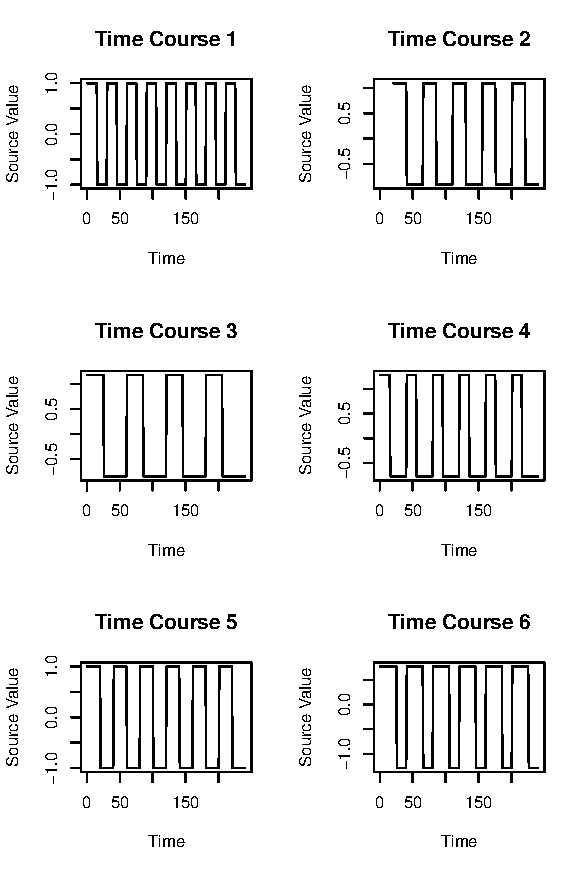
\includegraphics[scale=.59]{plots/1_1plots_3x2.pdf}\\
Normalising, while often confused with standardising, is very different. Standardising ensures the data has a unit variance and a mean of 0. Normalising the data rescales the values to $[0, 1]$. We do not want to do this as it will not make the data bias free and we want to maintain the current data scale.\\\\
\textbf{1.2}\\
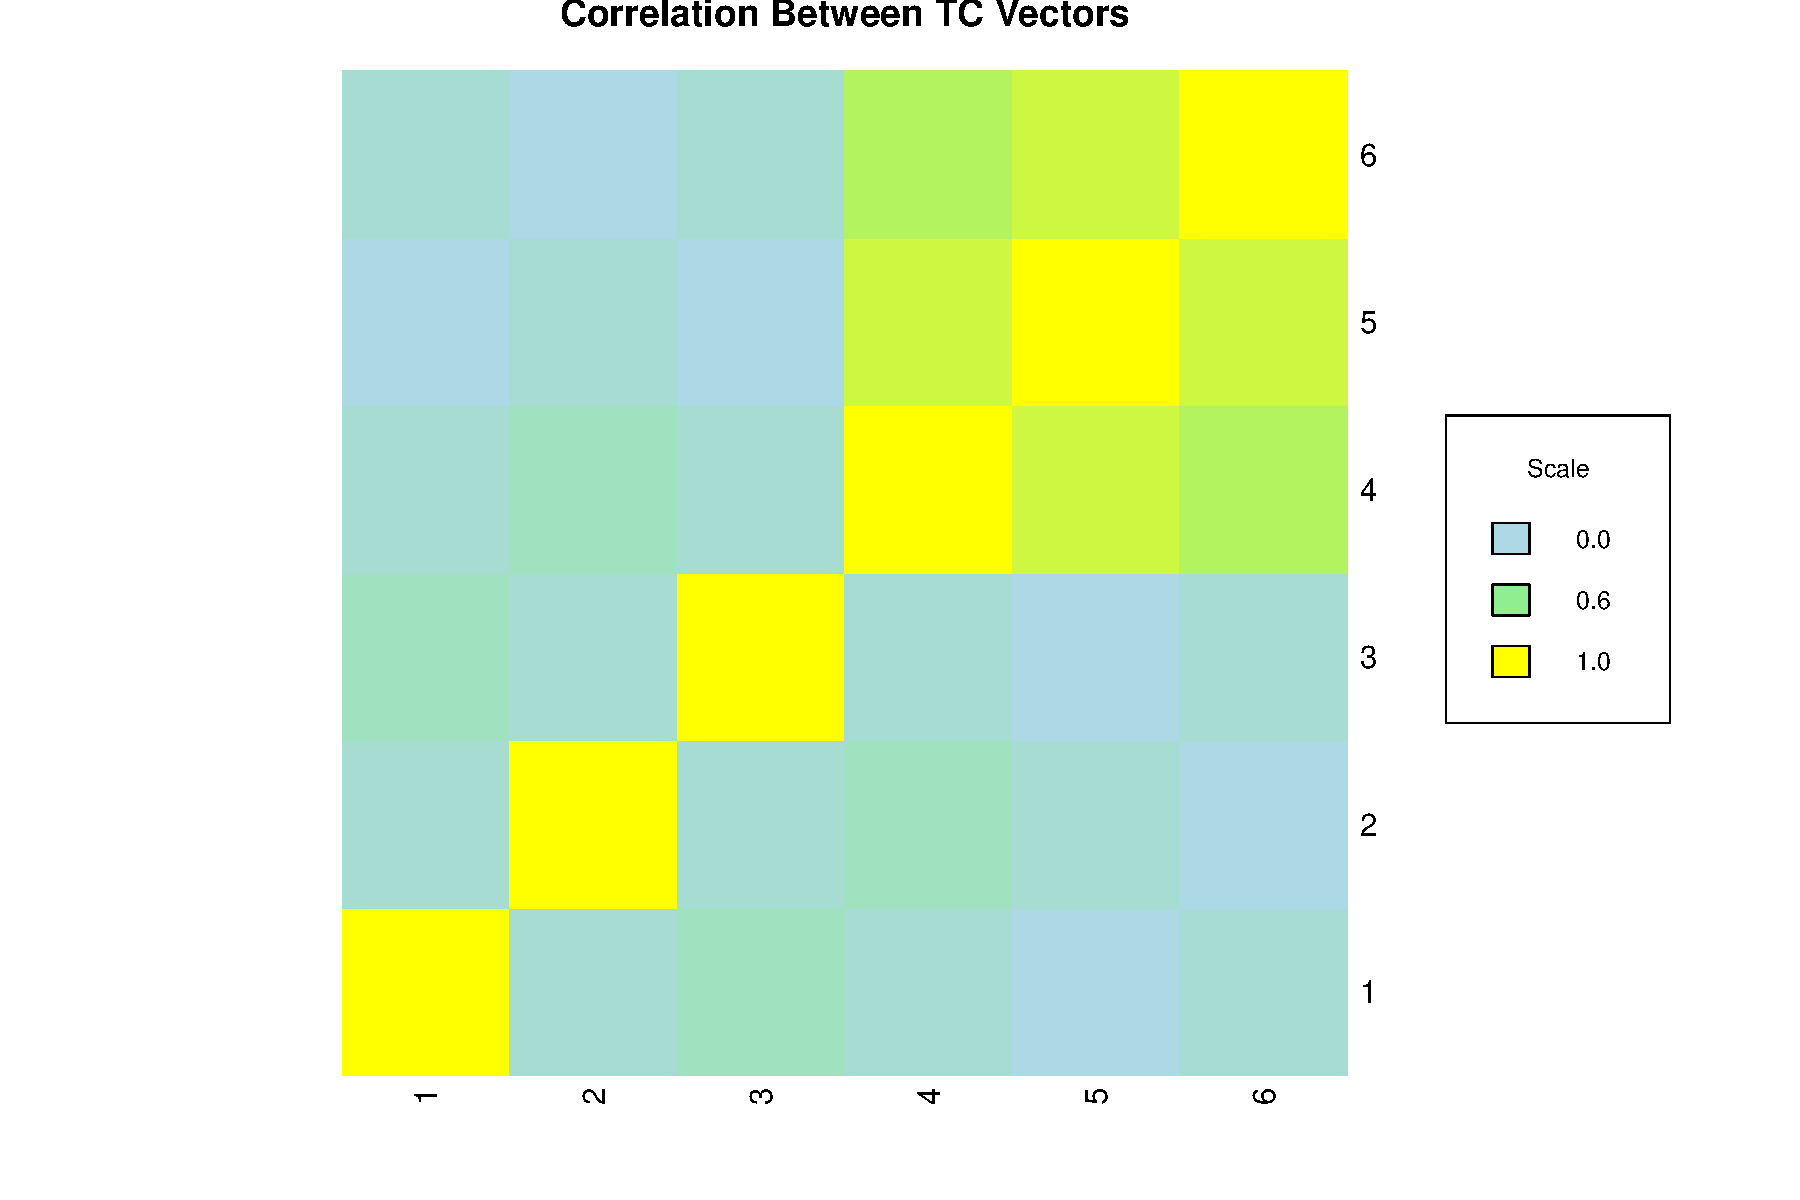
\includegraphics[scale=.35]{plots/corr_heatmap.pdf}\\
TCs 5 and 6 are highly correlated, and TCs 5 and 4 are verging on being correlated.\\
\textbf{1.3}\\
\begin{figure}[t]
\begin{subfigure}{.35\textwidth}
  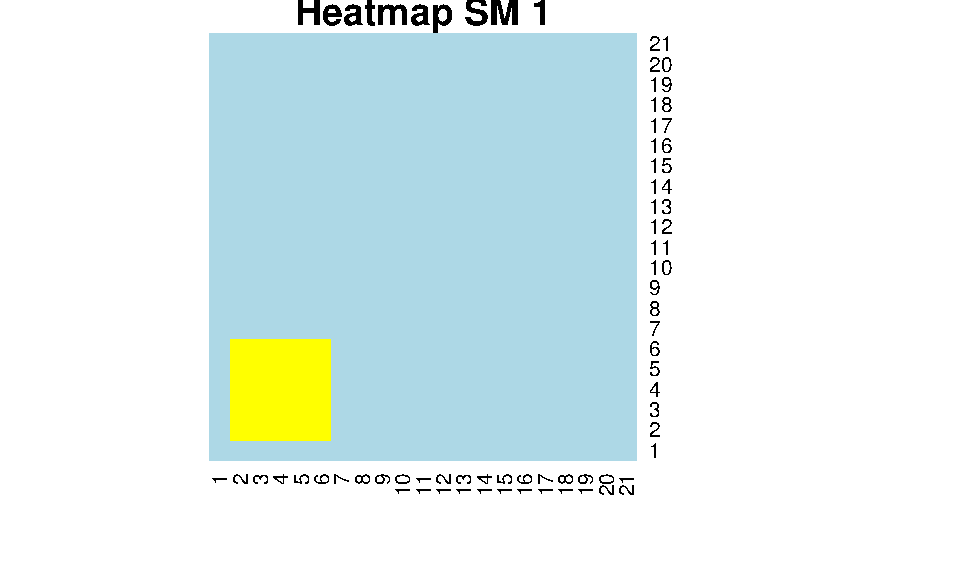
\includegraphics[width=.95\linewidth]{plots/SM1plot.pdf}
  \label{fig:sub1}
\end{subfigure}%
 \begin{subfigure}{.35\textwidth}
  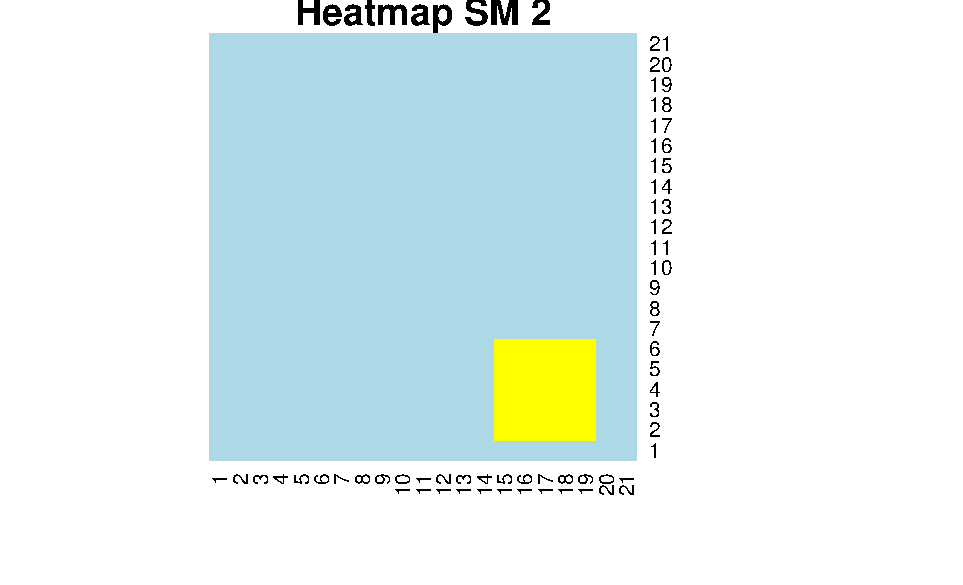
\includegraphics[width=.95\linewidth]{plots/SM2plot.pdf}
  \label{fig:sub1}
\end{subfigure}%
 \begin{subfigure}{.35\textwidth}
  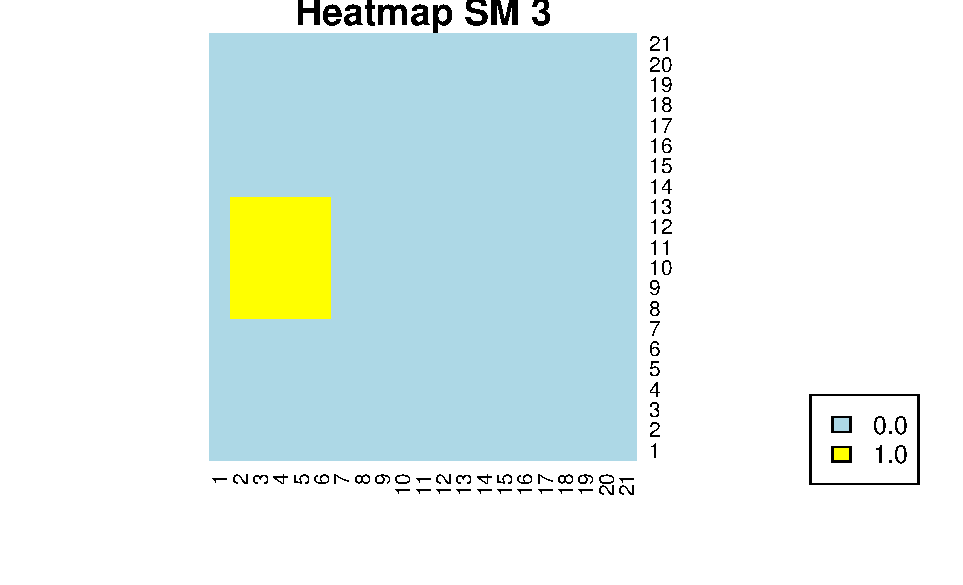
\includegraphics[width=.95\linewidth]{plots/SM3plot_legend.pdf}
  \label{fig:sub1}
\end{subfigure}%
\end{figure}
\begin{figure}[t]
\begin{subfigure}{.35\textwidth}
  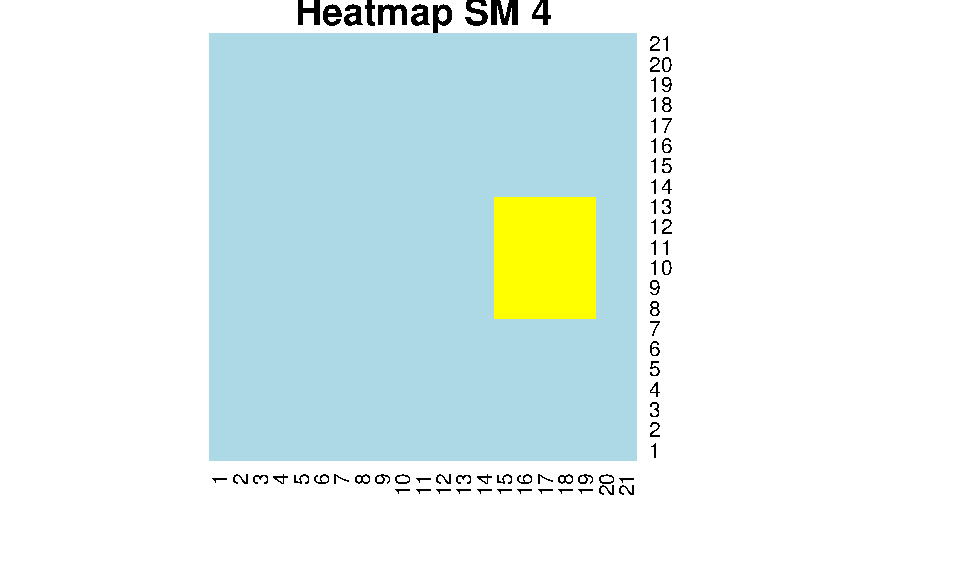
\includegraphics[width=.95\linewidth]{plots/SM4plot.pdf}
  \label{fig:sub1}
\end{subfigure}%
 \begin{subfigure}{.35\textwidth}
  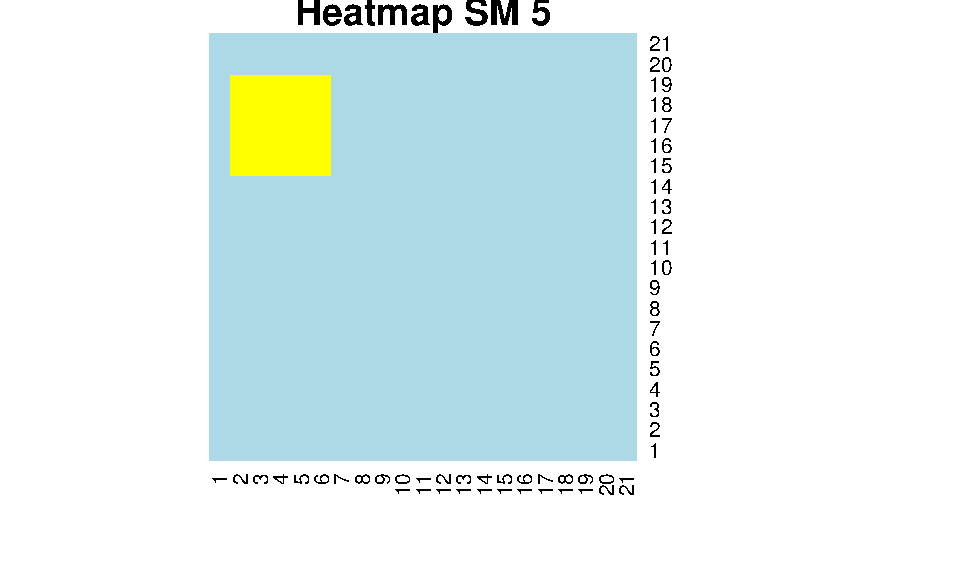
\includegraphics[width=.95\linewidth]{plots/SM5plot.pdf}
  \label{fig:sub1}
\end{subfigure}%
 \begin{subfigure}{.35\textwidth}
  \includegraphics[width=.95\linewidth]{plots/SM6plot_legend.pdf}
  \label{fig:sub1}
\end{subfigure}%
\end{figure}
Showing if these six SMs are independent: \\\\
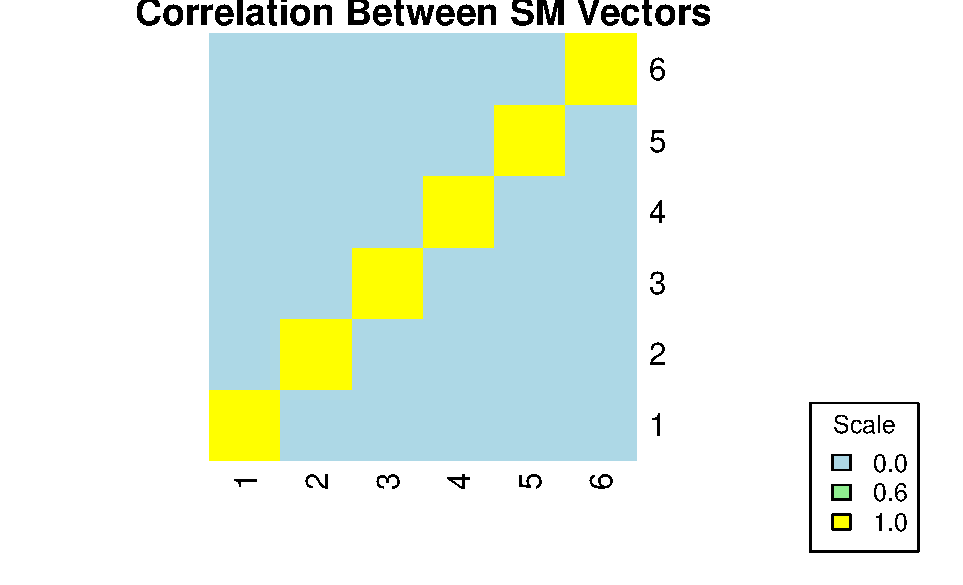
\includegraphics[width=.55\linewidth]{plots/SM_correlations.pdf}
\\
There appears to be no correlation between SM vectors.\\
Standardisation is not important as the SM vectors all have the same distribution of values, it is just their position in the vector that differ. Hence all of their means and variances are very similar.\\\\
\textbf{1.4}\\
 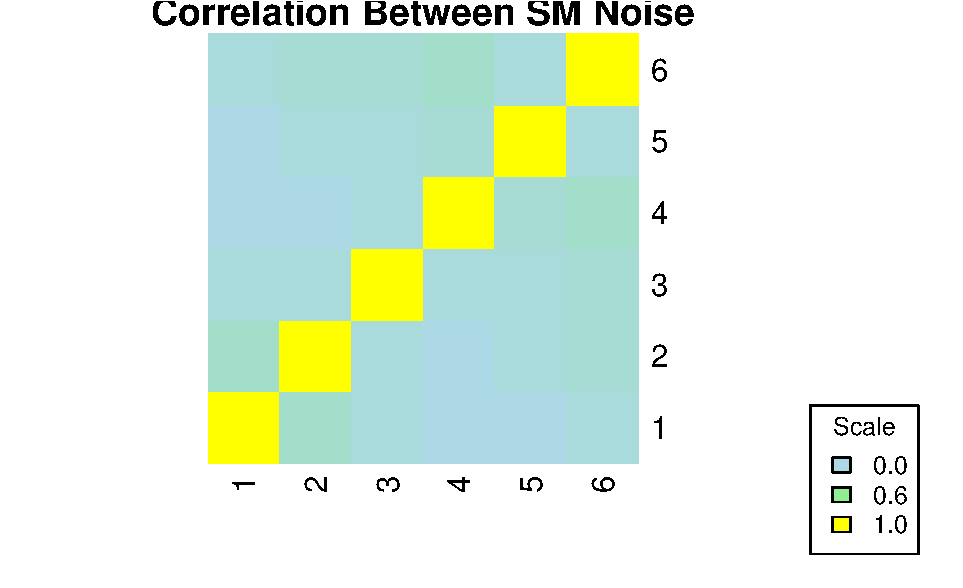
\includegraphics[width=.55\linewidth]{plots/SM_noise_corr.pdf}
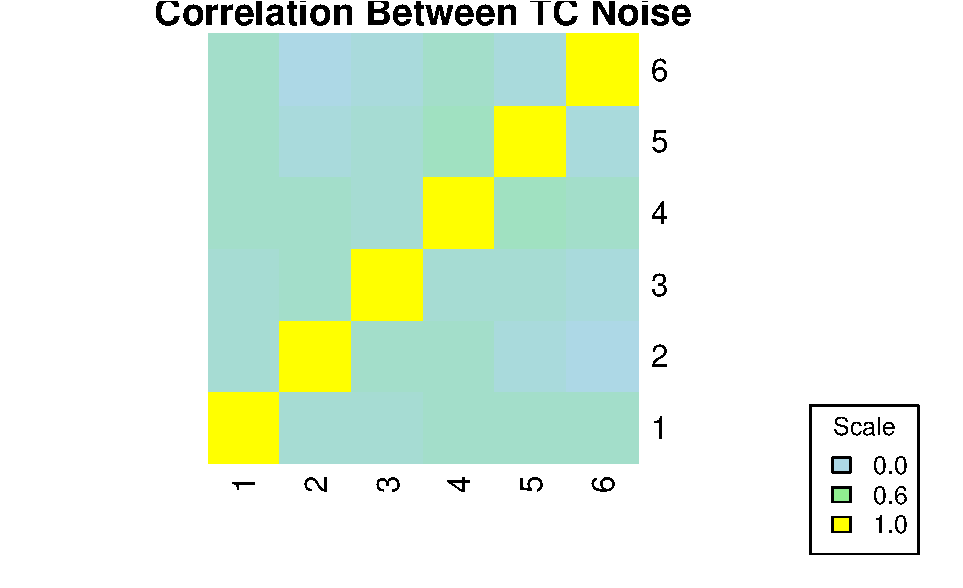
\includegraphics[width=.55\linewidth]{plots/corr_TC_noise.pdf}

The noise does not look correlated across sources.\\
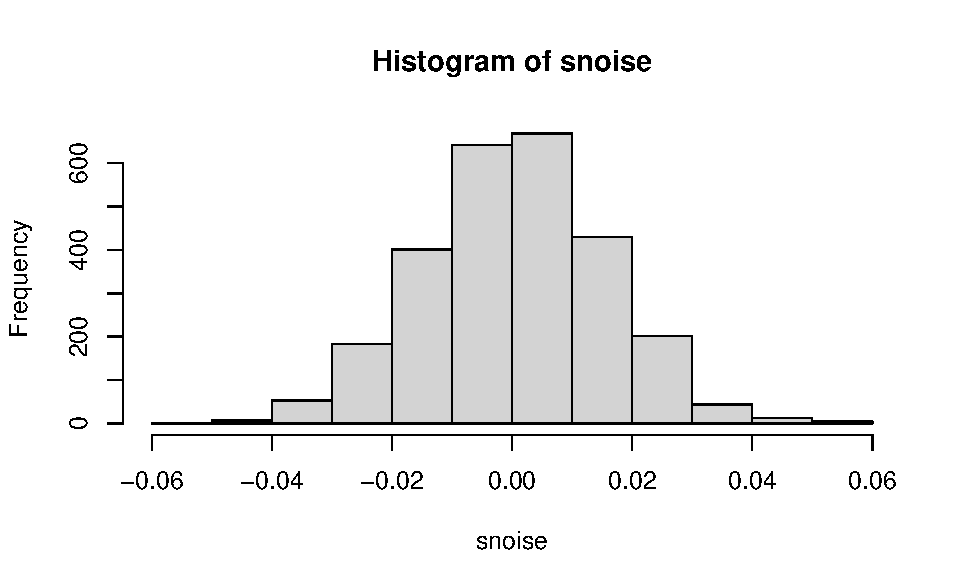
\includegraphics[width=.55\linewidth]{plots/hist_snoise.pdf}
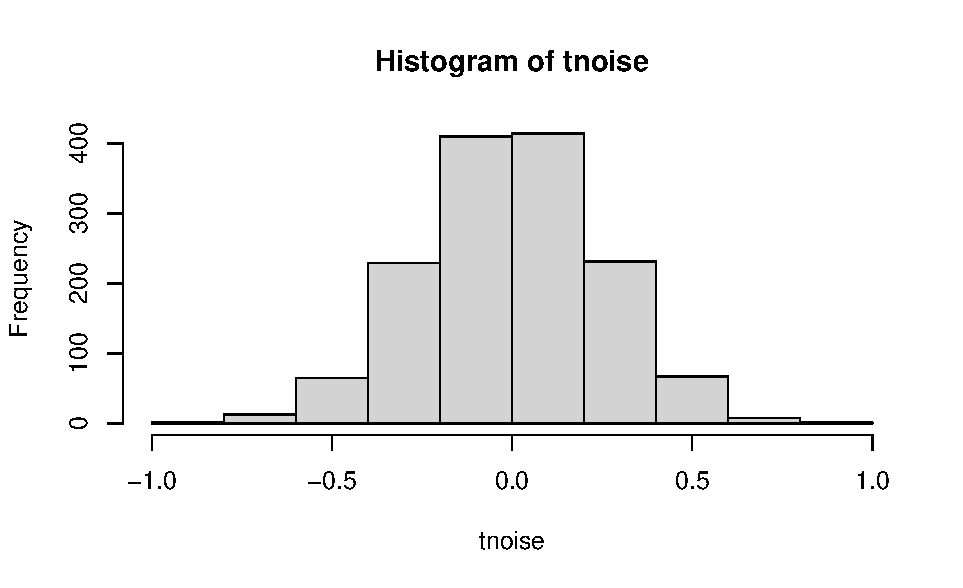
\includegraphics[width=.55\linewidth]{plots/hist_tnoise.pdf}
\\
These distributions appear normal and reflect the distributions of $\sim$N(0, 0.015) and $\sim$N(0, 0.25) respectively.\\\\
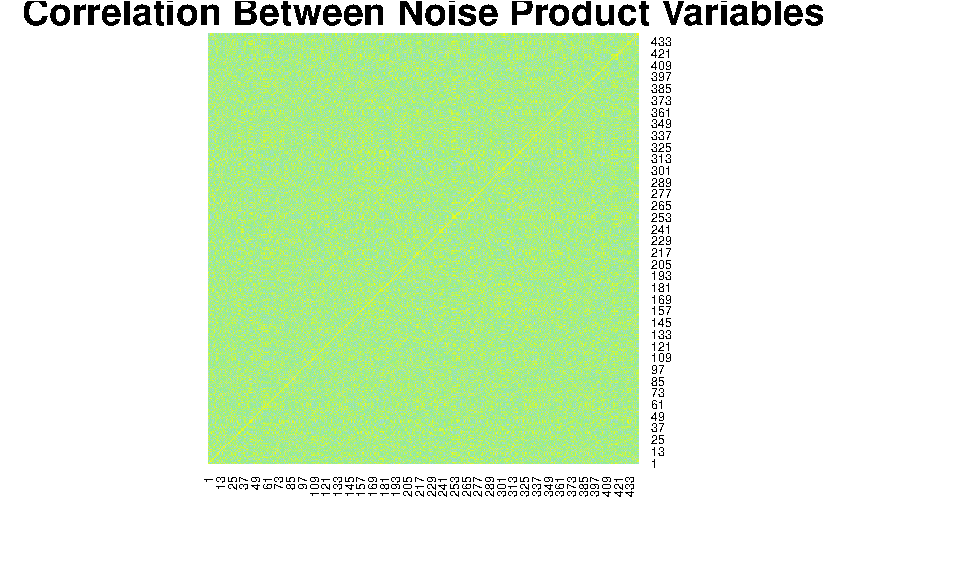
\includegraphics[width=.75\linewidth]{plots/Product_noise_heatmap.pdf}
\\While this is a very granular heatmap, there is evidence of some correlation across the V number of variables with the product of the noise types.\\\\
\textbf{1.5}\\
These products could exist if the noise matricies were transposed. In which case the resulting calculation
\begin{lstlisting}
X = (TC %*% t(TC_noise)) %*% (SM %*% t(SM_noise))
\end{lstlisting} would have non-conforming dimensions. Typically, noise is only multiplicative if the noise is correlated with the data; in this case, it is not. Hence additive noise is okay. \\
I have included two plots of 100 randomly selected time-series from $\textbf{X}$:\\
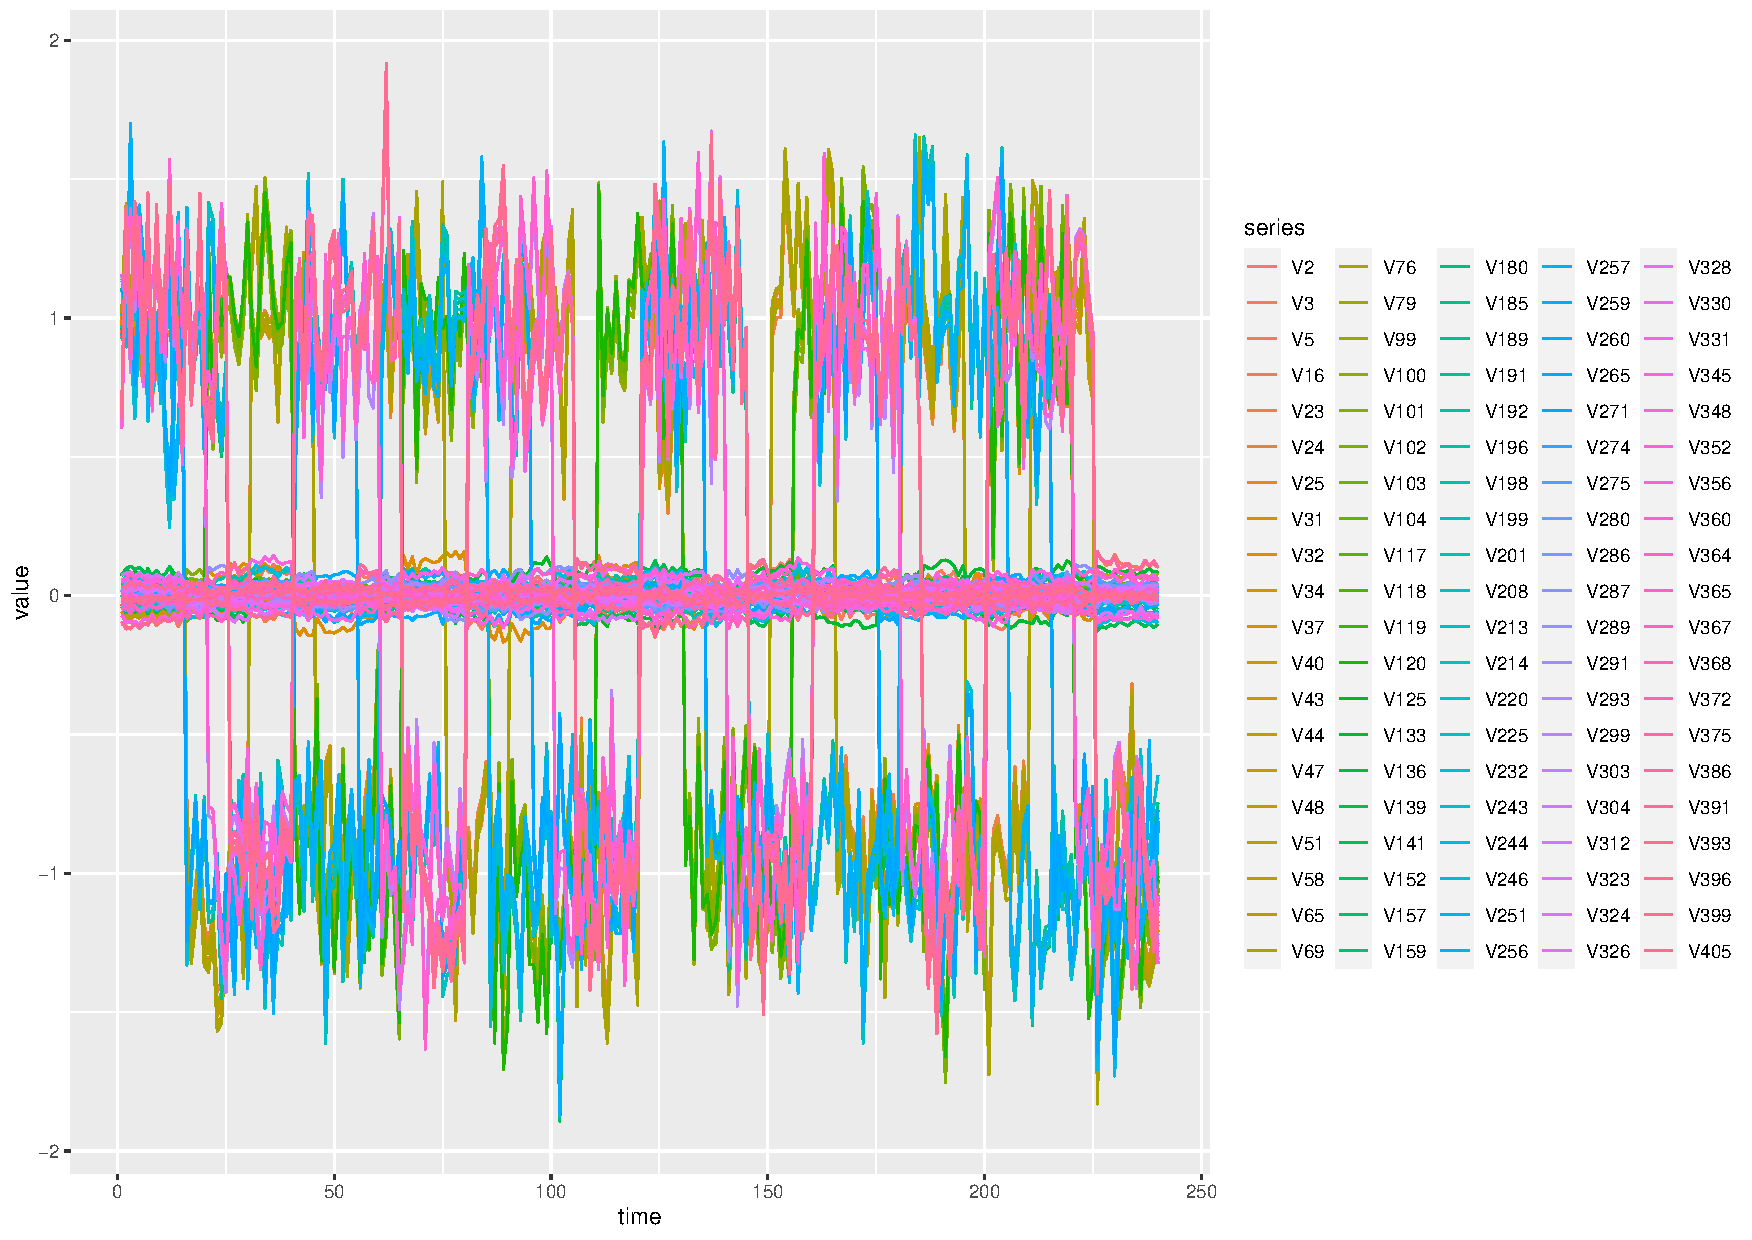
\includegraphics[width=.75\linewidth]{plots/wild_15plot.pdf}\\
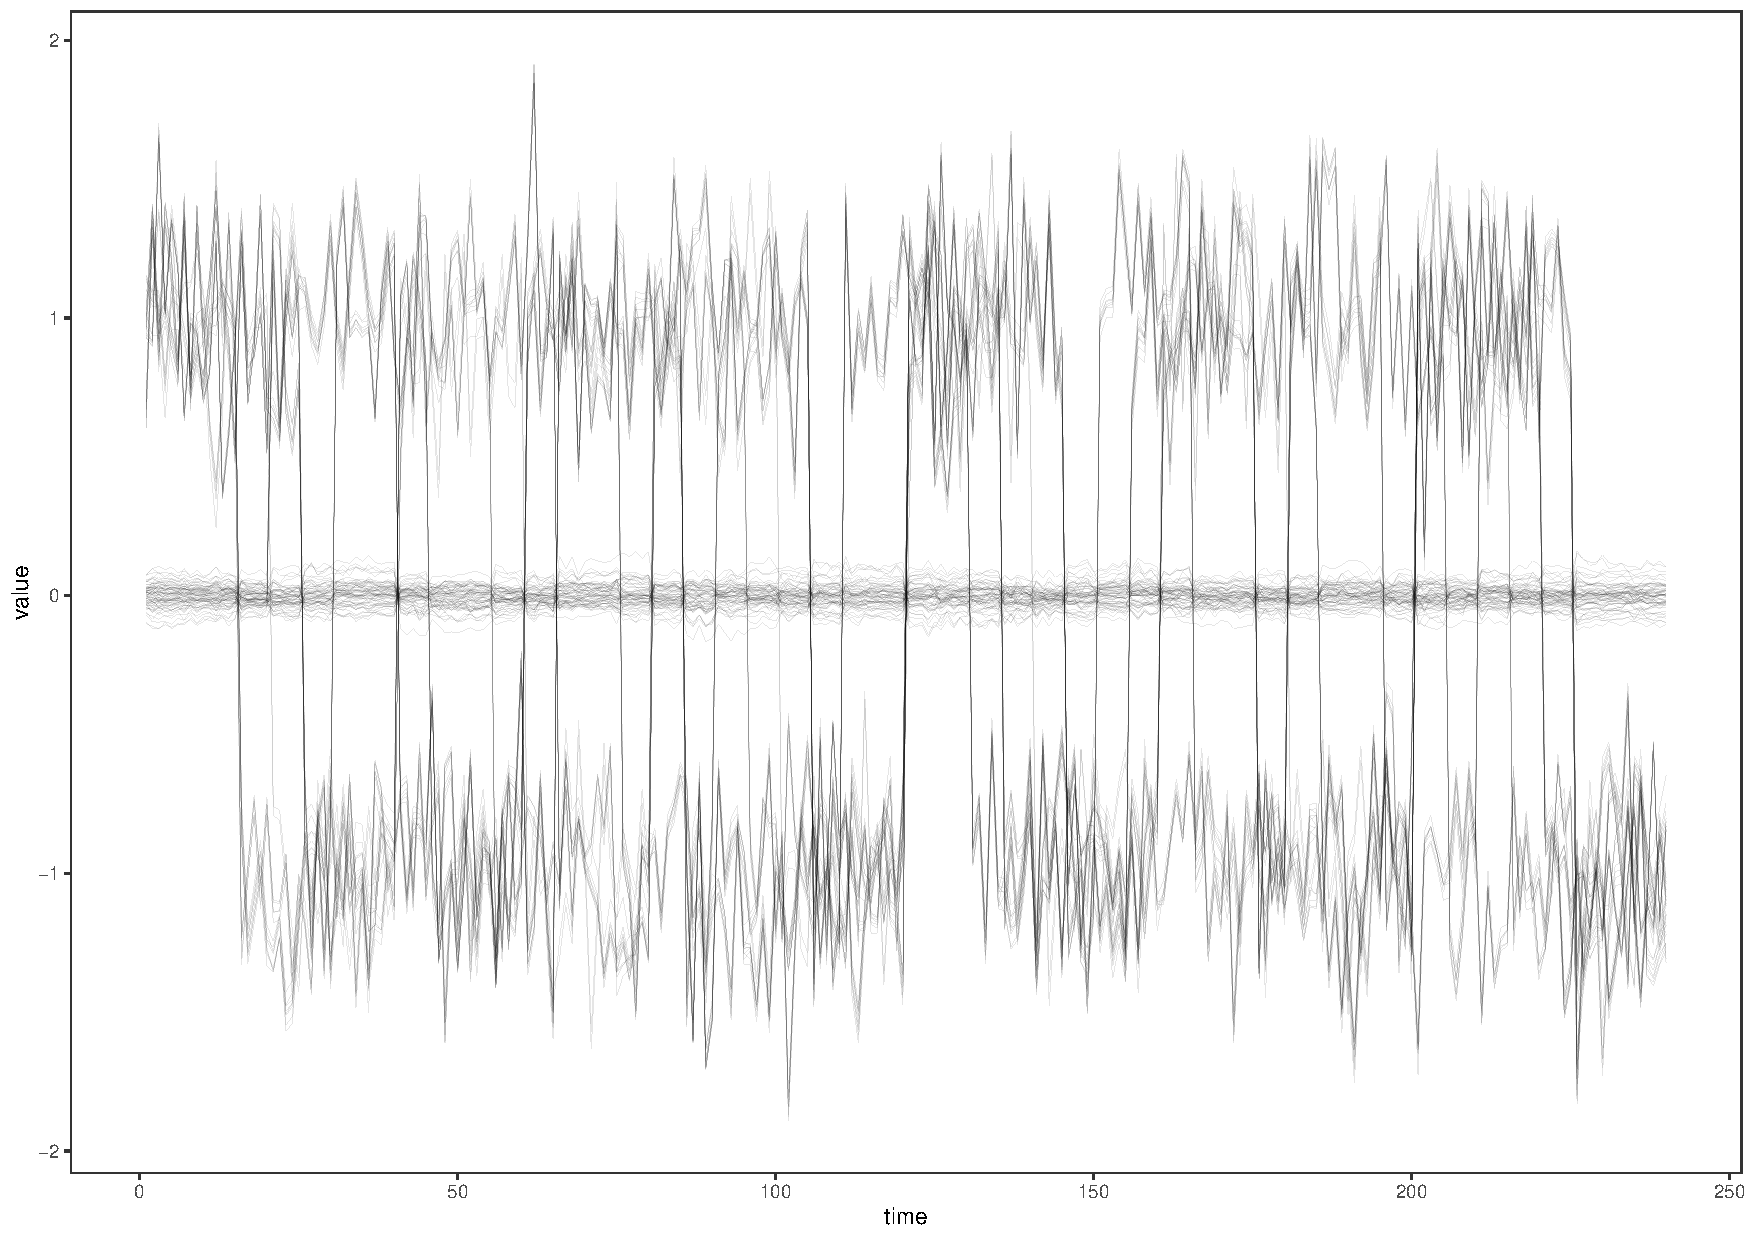
\includegraphics[width=.55\linewidth]{plots/15plot.pdf}\\
A plot of the variance of the 411 variables:\\
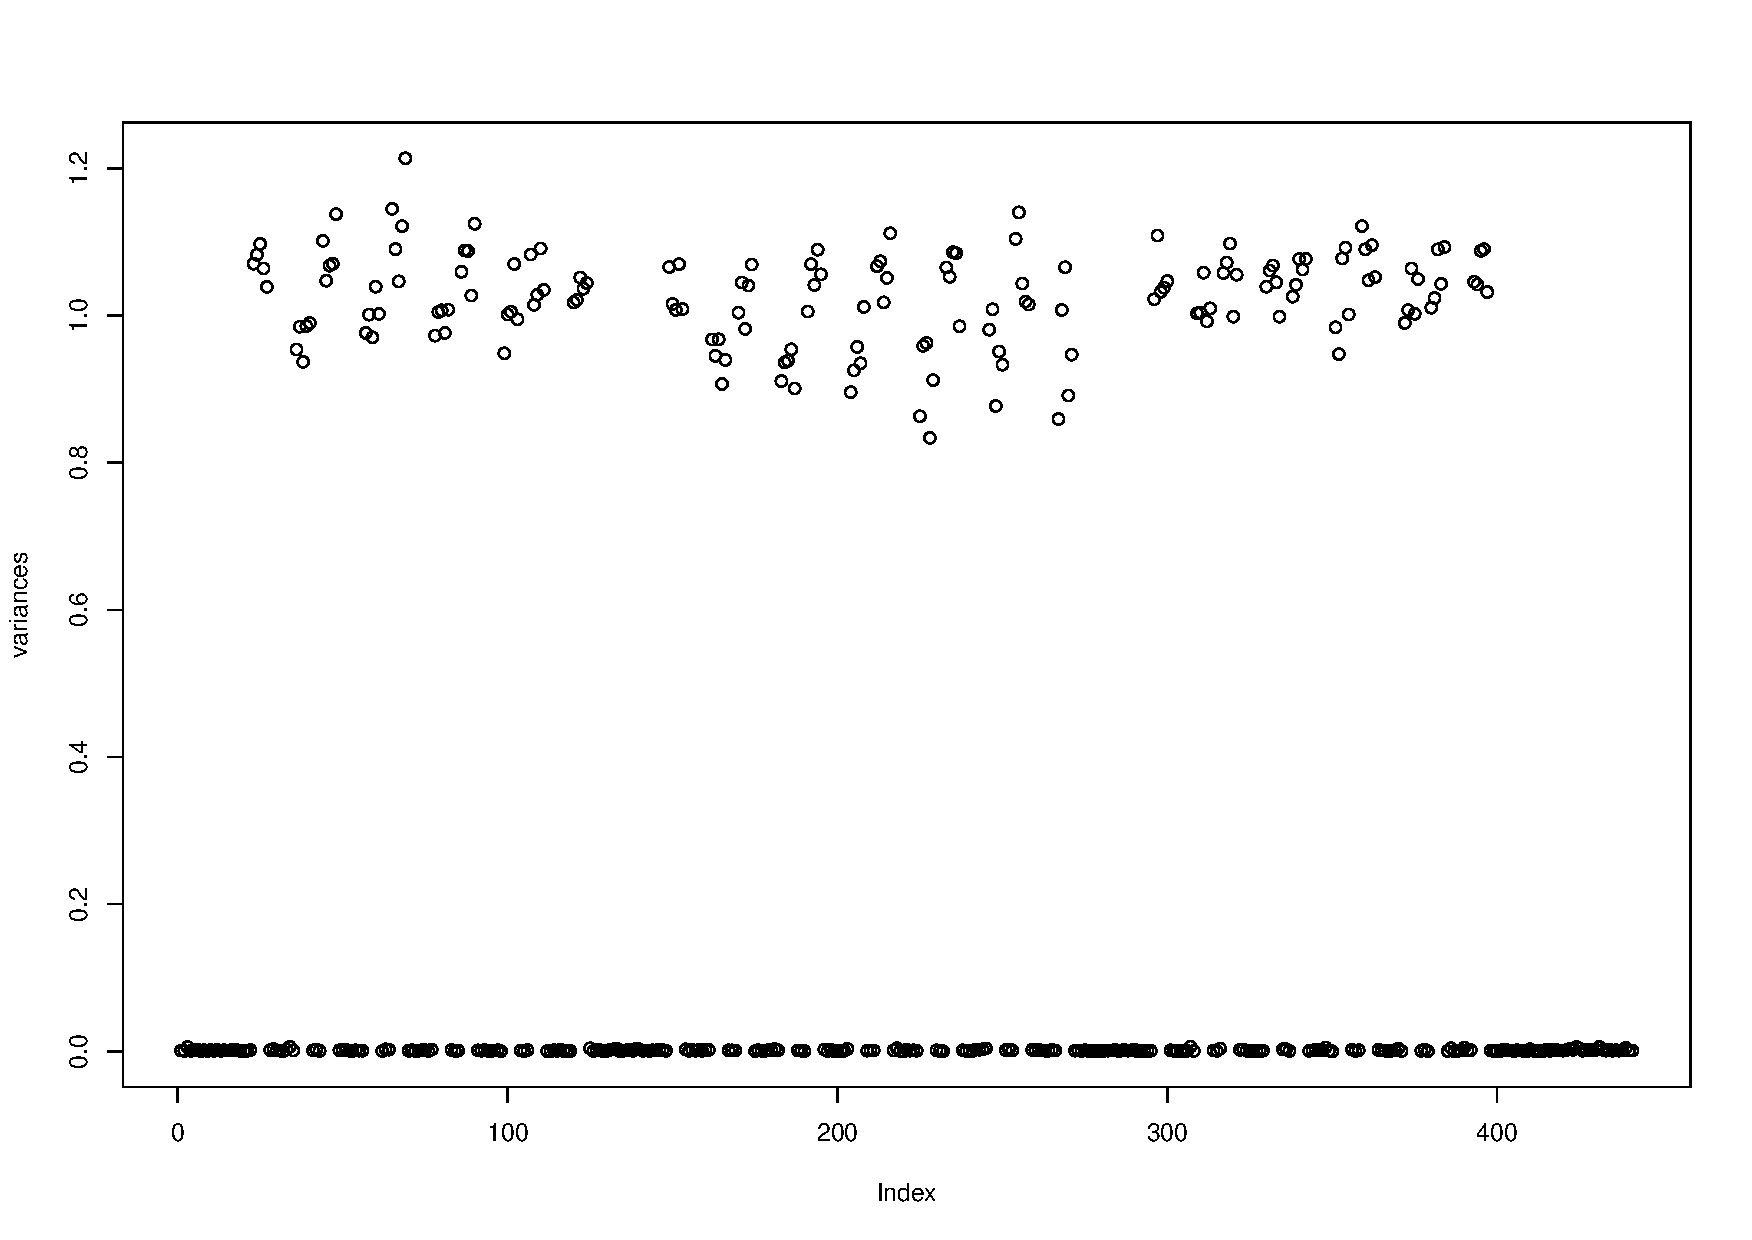
\includegraphics[width=.55\linewidth]{plots/variance_plot15.pdf}\\
The variance plot displays some interesting information. There are two main clusters, variances of value $\sim$1, and of value 0.\\\\
\textbf{Question 2.}\\\\
\textbf{2.1}\\
$\textbf{A}_{LSR}$ and $\textbf{D}_{LSR}$ retrieved sources plotted side by side:\\\\
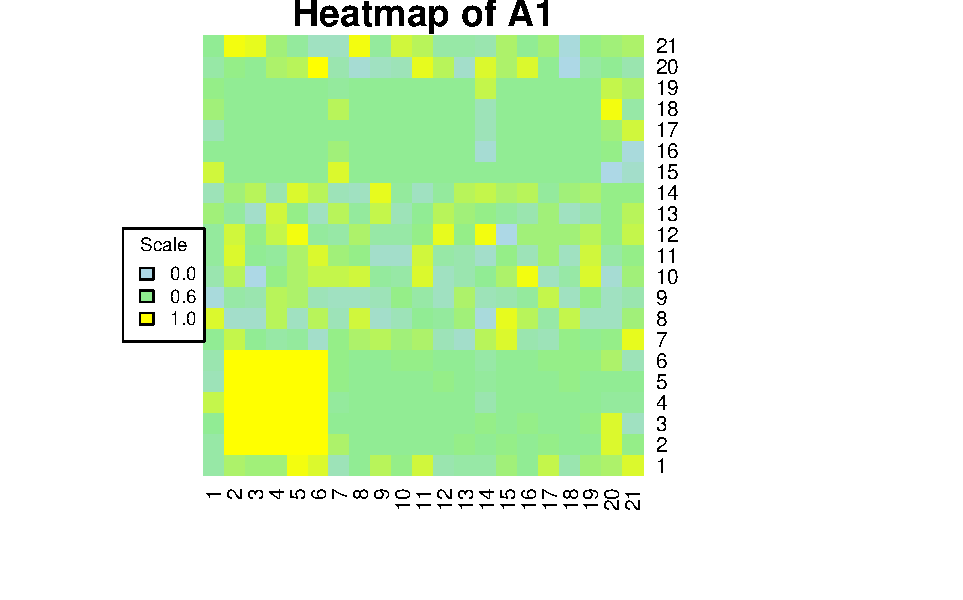
\includegraphics[width=.45\linewidth]{plots/A1_heatmap.pdf}
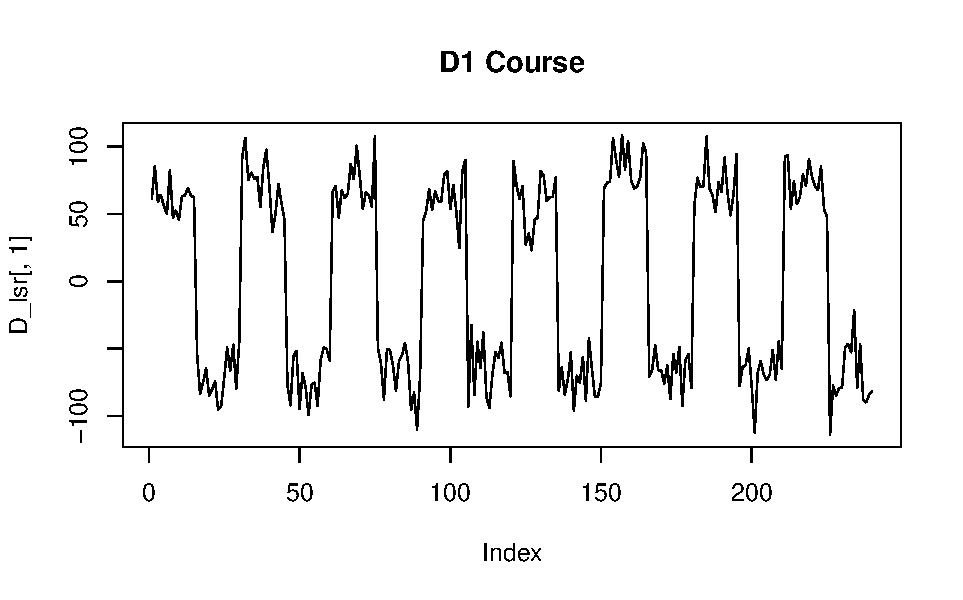
\includegraphics[width=.45\linewidth]{plots/D1_line.pdf}\\

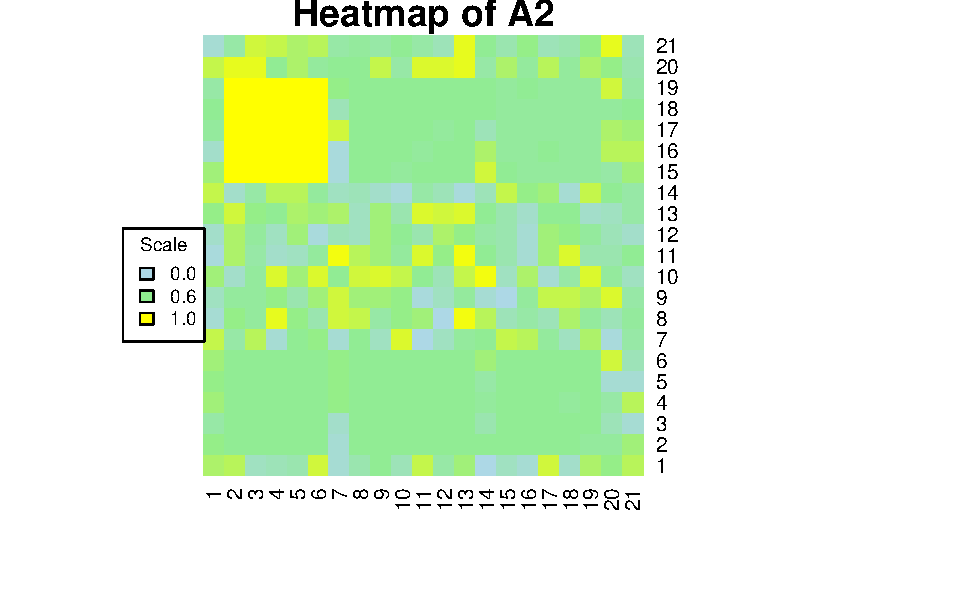
\includegraphics[width=.45\linewidth]{plots/A2_heatmap.pdf}
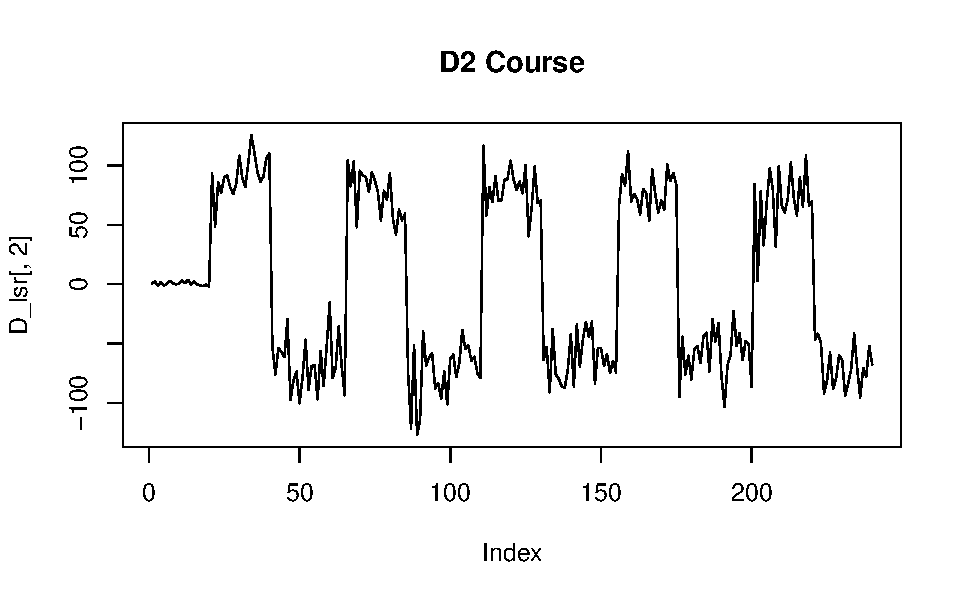
\includegraphics[width=.45\linewidth]{plots/D2_line.pdf}\\

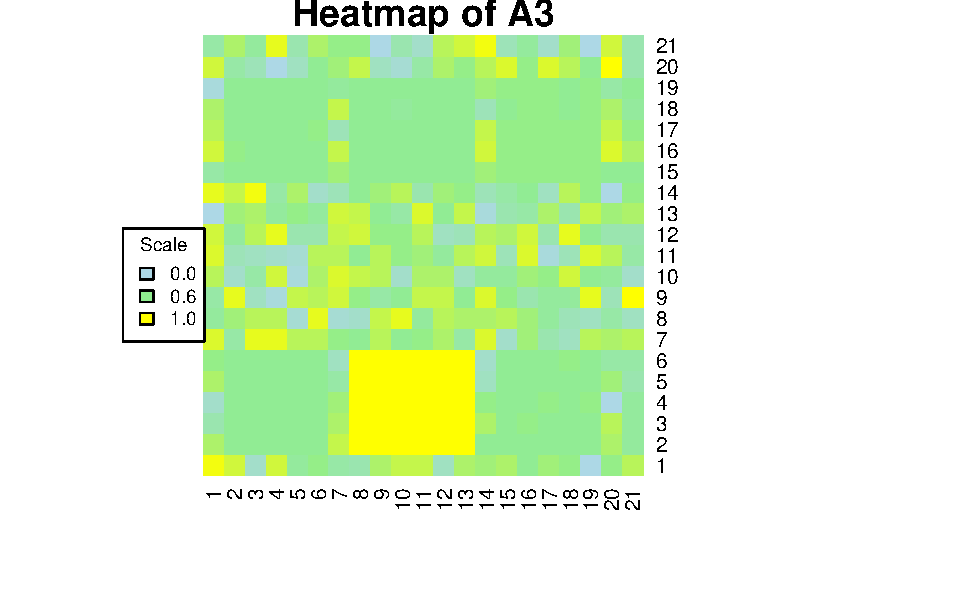
\includegraphics[width=.45\linewidth]{plots/A3_heatmap.pdf}
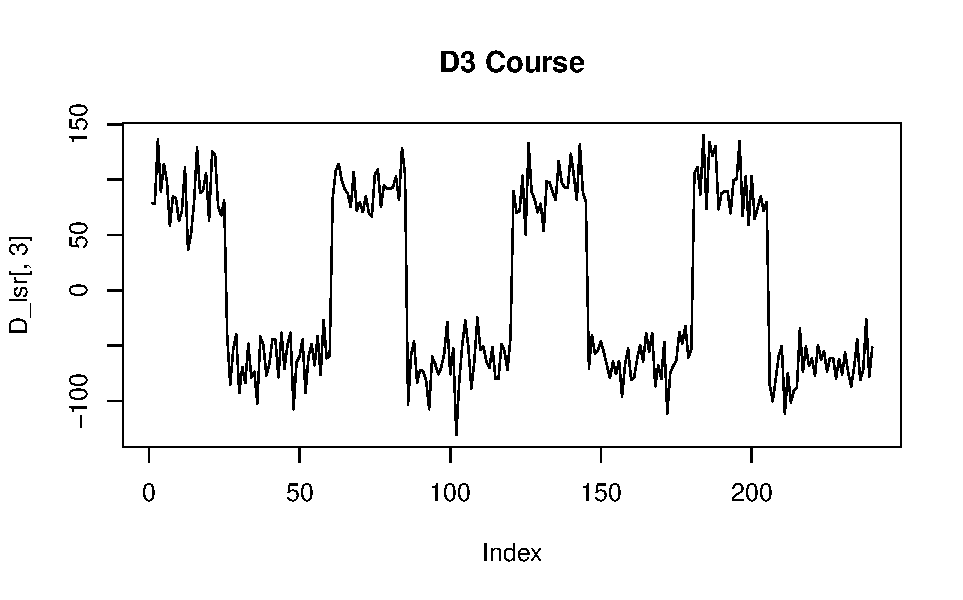
\includegraphics[width=.45\linewidth]{plots/D3_line.pdf}\\

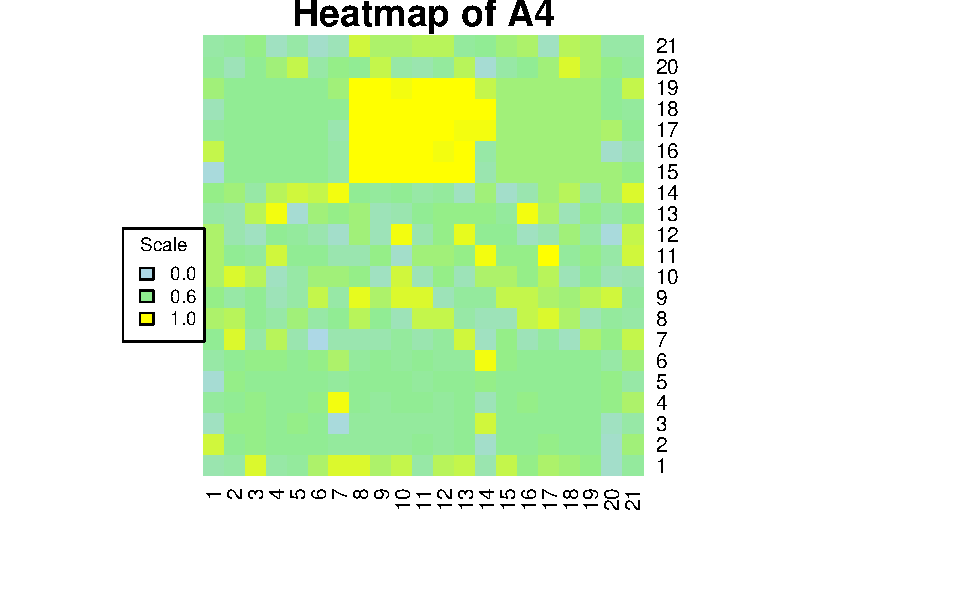
\includegraphics[width=.45\linewidth]{plots/A4_heatmap.pdf}
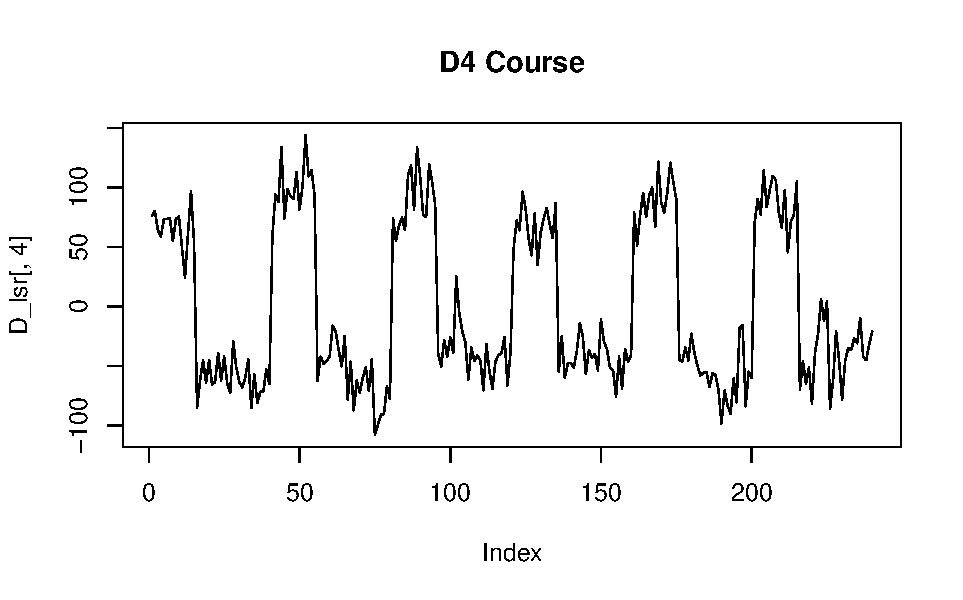
\includegraphics[width=.45\linewidth]{plots/D4_line.pdf}\\

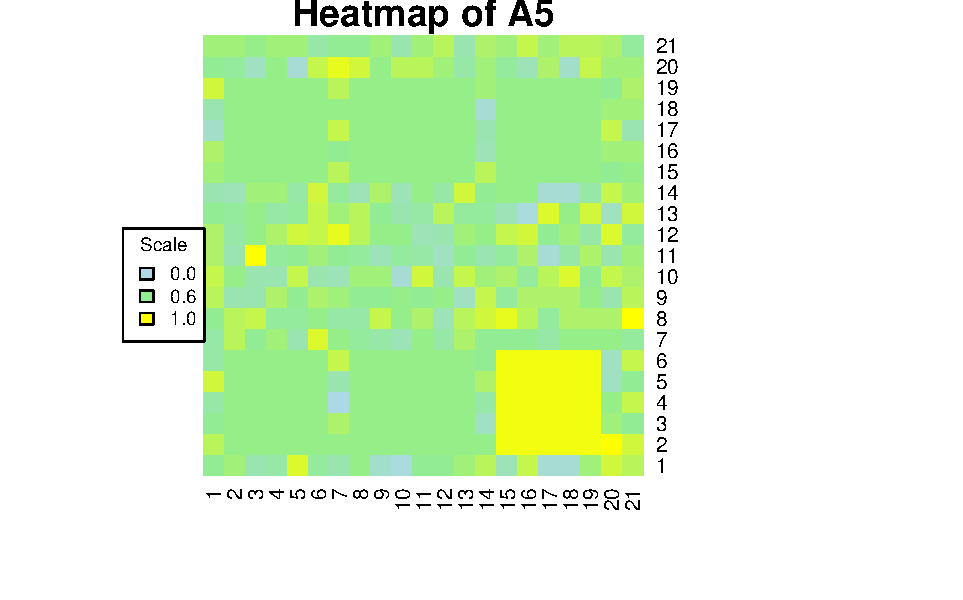
\includegraphics[width=.45\linewidth]{plots/A5_heatmap.pdf}
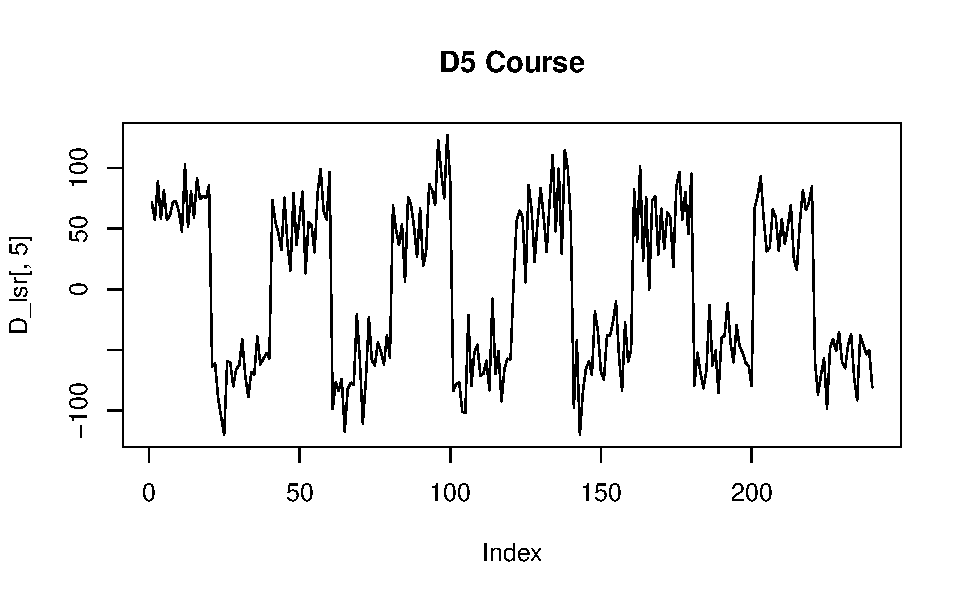
\includegraphics[width=.45\linewidth]{plots/D5_line.pdf}\\

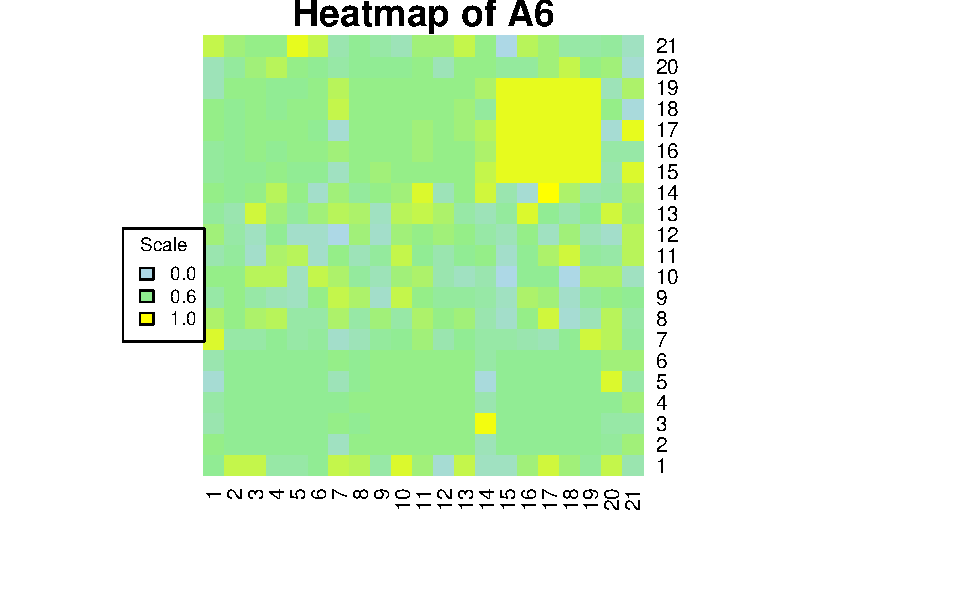
\includegraphics[width=.45\linewidth]{plots/A6_heatmap.pdf}
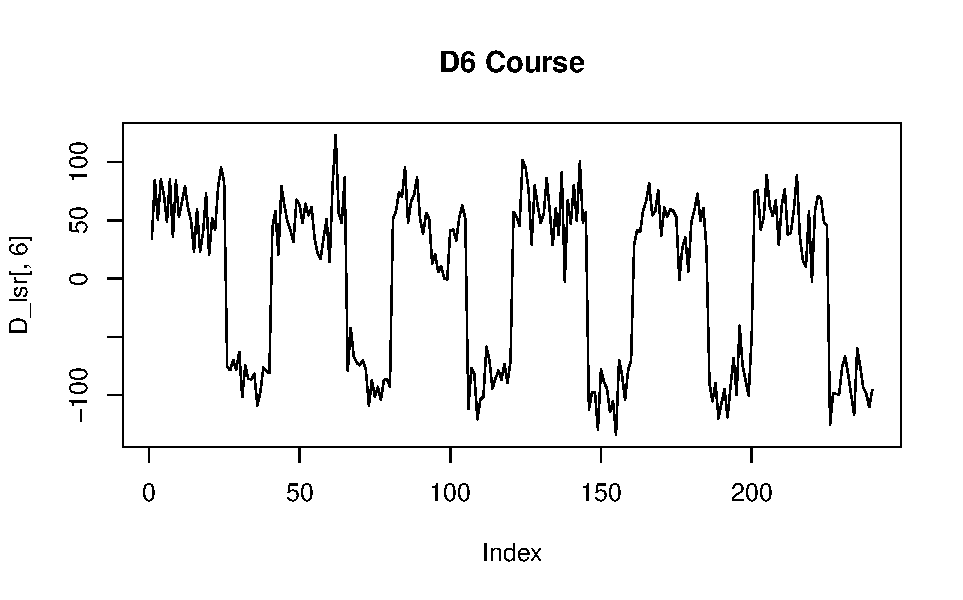
\includegraphics[width=.45\linewidth]{plots/D6_line.pdf}\\\\
Scatter plot between the $3rd$ column of $\textbf{D}_{LSR}$ and the $30th$ column of standardized \textbf{X}:\\
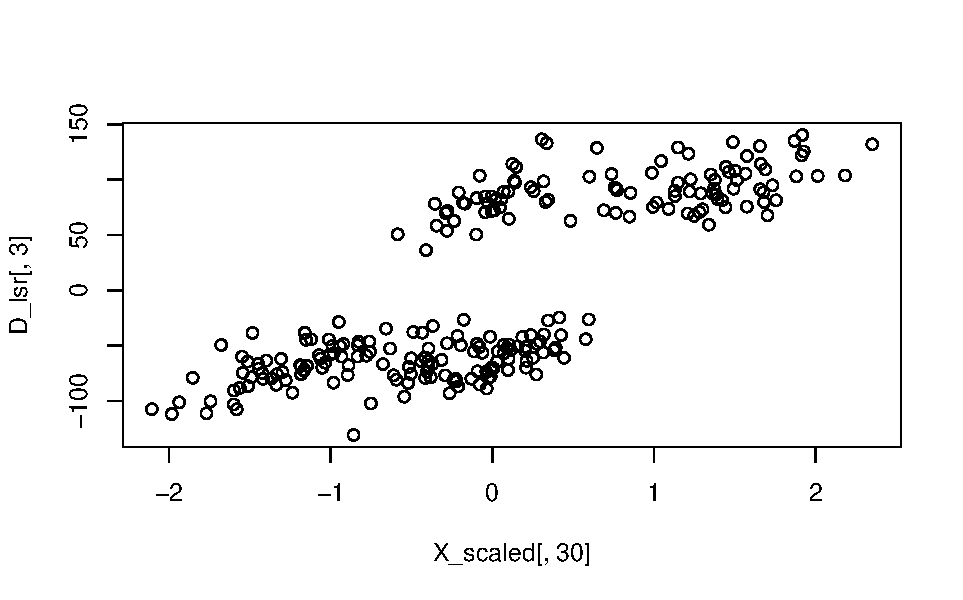
\includegraphics[width=.65\linewidth]{plots/d3_X_scatter.pdf}\\
When compared to the relationship the $4th$ column of $\textbf{D}_{LSR}$ has with \textbf{X}:\\
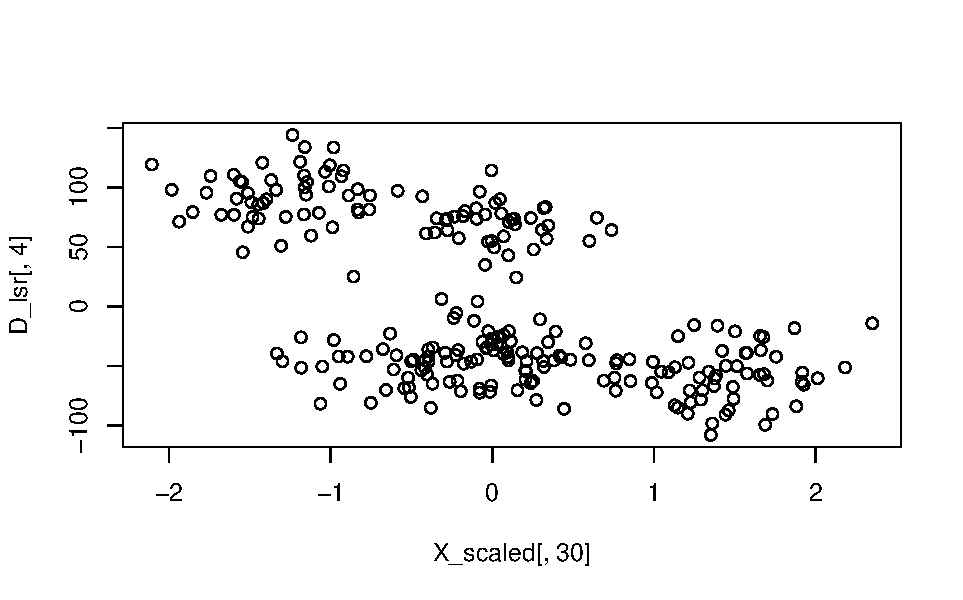
\includegraphics[width=.65\linewidth]{plots/scatter_d4_x.pdf}\\
You can see there appears to be a more linear relationship in the first plot. This is due to the $30th$ column of \textbf{X} being constructed by the third $\textbf{TC}$. As $\textbf{D}_{LSR}$ is an estimate of $\textbf{TC}$, this relationship is carried through and hence a more linear relationship is shown between \textbf{X} and $\textbf{D}_{LSR}$'s third column than fourth.\\\\
\textbf{2.2}\\
The sum of the $C_{TRR}$ is greater than the sum of $C_{TLSR}$:
\begin{lstlisting}
c(sum(c_trr), sum(c_tlsr))
\end{lstlisting}
\begin{alltt}
\input{2_2_ctrr}
\end{alltt}
Now for $\lambda = 1000$:\\
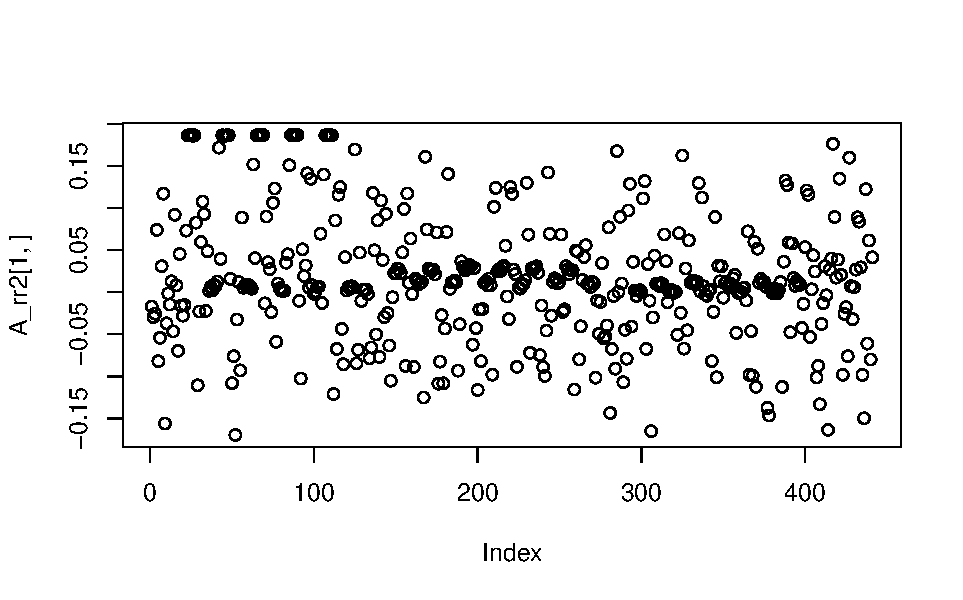
\includegraphics[width=.45\linewidth]{plots/2_2_Arr.pdf}
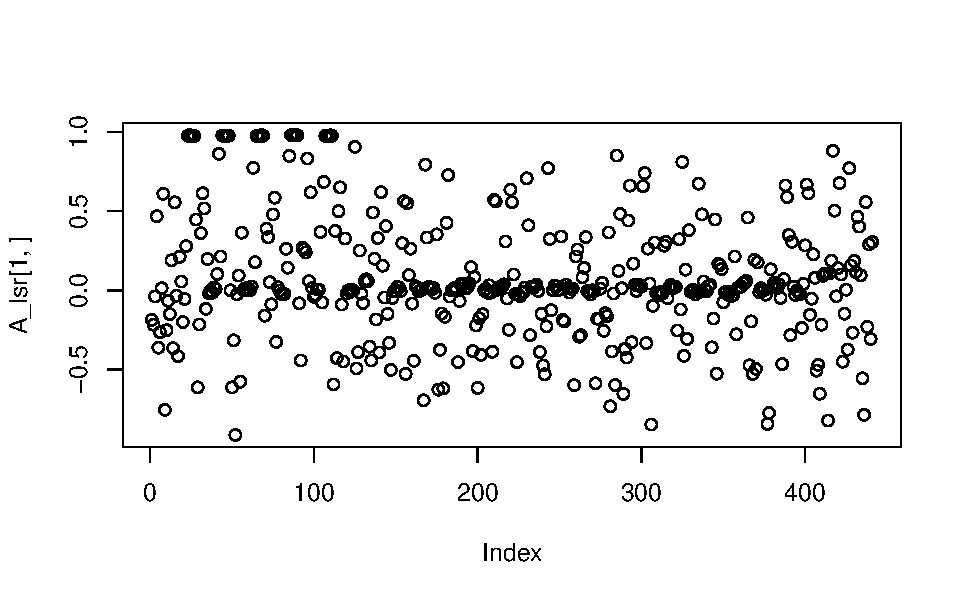
\includegraphics[width=.45\linewidth]{plots/2_2_A_lsr.pdf}\\
These graphs show there is a majority of datapoints at 0.\\\\
\textbf{2.3}\\
The code to produce the MSEs through Lasso Regression that was used is from the Assignment sheet and translated into R.\\
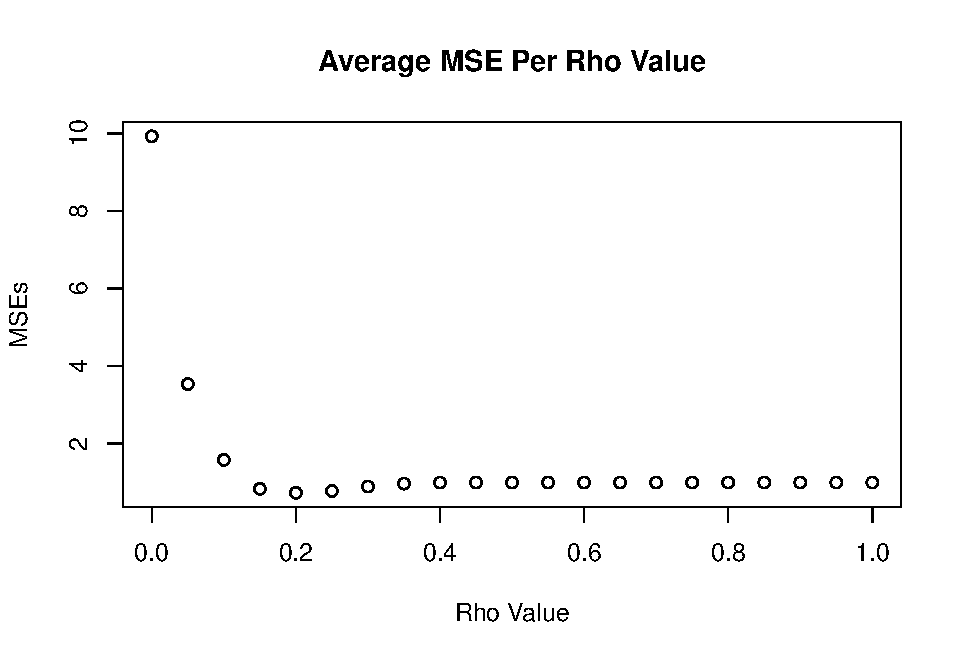
\includegraphics[width=.65\linewidth]{plots/2_3_rho_min_is_0_2.pdf}\\
The minimum $\rho$ is $0.2$. $LR$ diverged at $\rho$ value of $0.4$. Hence I will be choosing $\rho$ = $0.2$. Whether or not this was an appropriate decision is addressed in question \textbf{2.4}.\\
\textbf{2.4}\\
\begin{lstlisting}
#i TC and DRR
C_trr = cor(TC, D_rr)
#i SM and Arr
C_srr = cor(SM, t(A_rr))
#i TC Dlr
C_tlr = cor(TC, D_lr)
#i TC and DRR
C_slr = cor(SM, t(A_lr))

c(sum(C_tlr), sum(C_trr)) 
c(sum(C_slr), sum(C_srr)) 
\end{lstlisting}
\begin{alltt}
\input{2_4_code}
\end{alltt}
My $C_{TLR} < C_{TRR} $ which is not supposed to happen, however my $C_{SLR} > C_{SRR} $ which is in-line with the expected outcome. Hence my $\rho$ value, while producing the minimum MSE, may not have been the best choice of value.\\\\
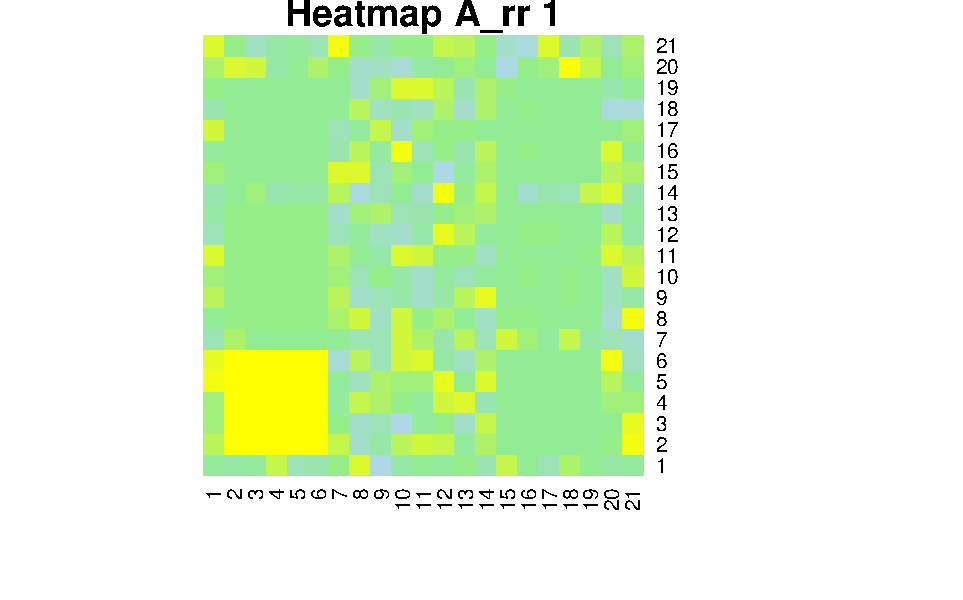
\includegraphics[width=.25\linewidth]{plots/Rplot.pdf}
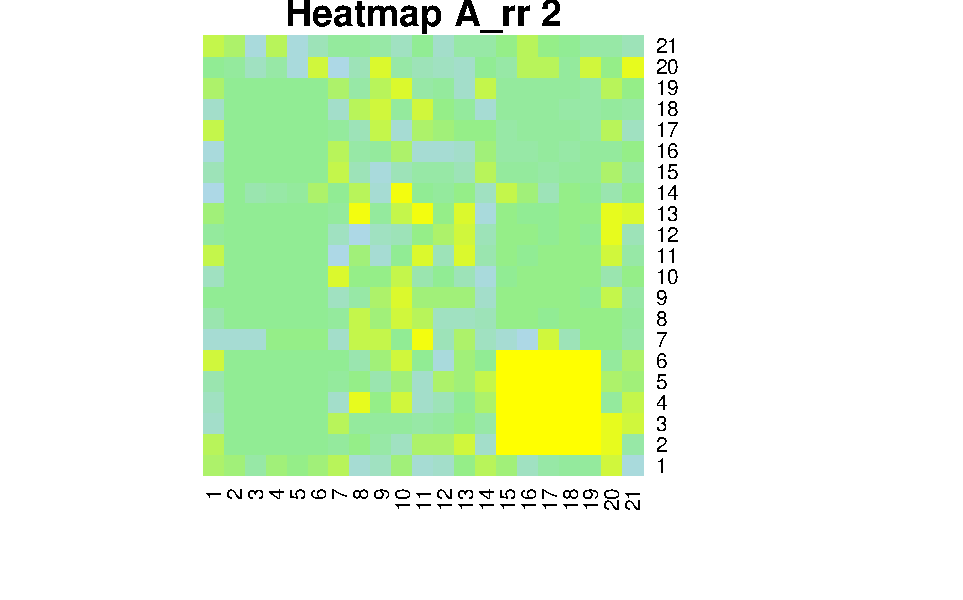
\includegraphics[width=.25\linewidth]{plots/arr2.pdf}
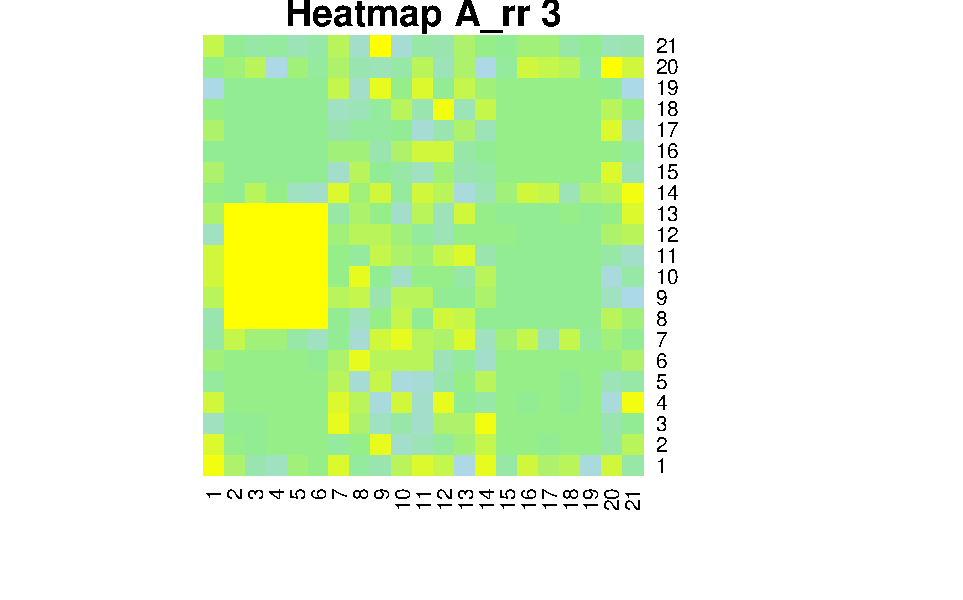
\includegraphics[width=.25\linewidth]{plots/arr3.pdf}
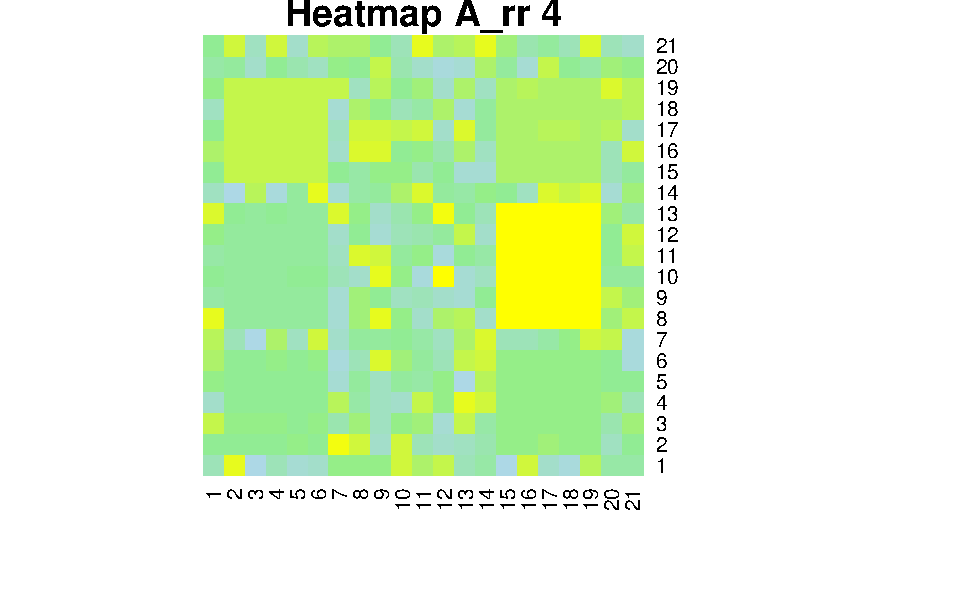
\includegraphics[width=.25\linewidth]{plots/arr4.pdf}\\
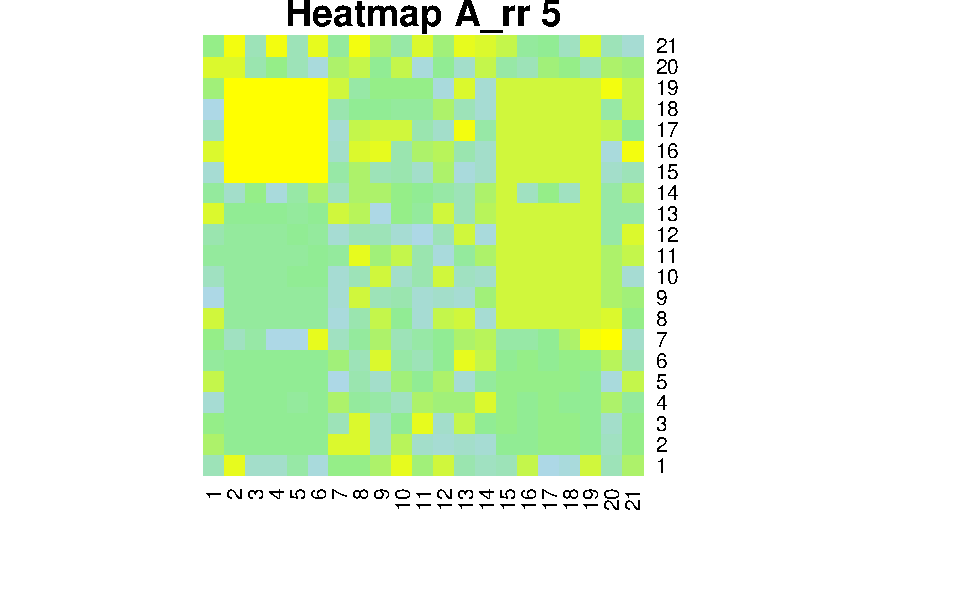
\includegraphics[width=.25\linewidth]{plots/arr5.pdf}
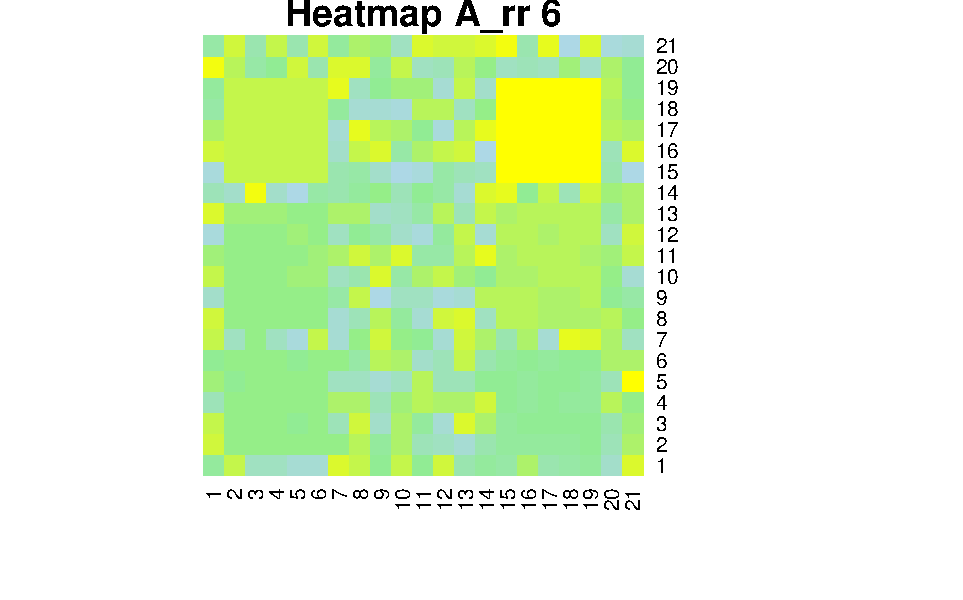
\includegraphics[width=.25\linewidth]{plots/arr6.pdf}
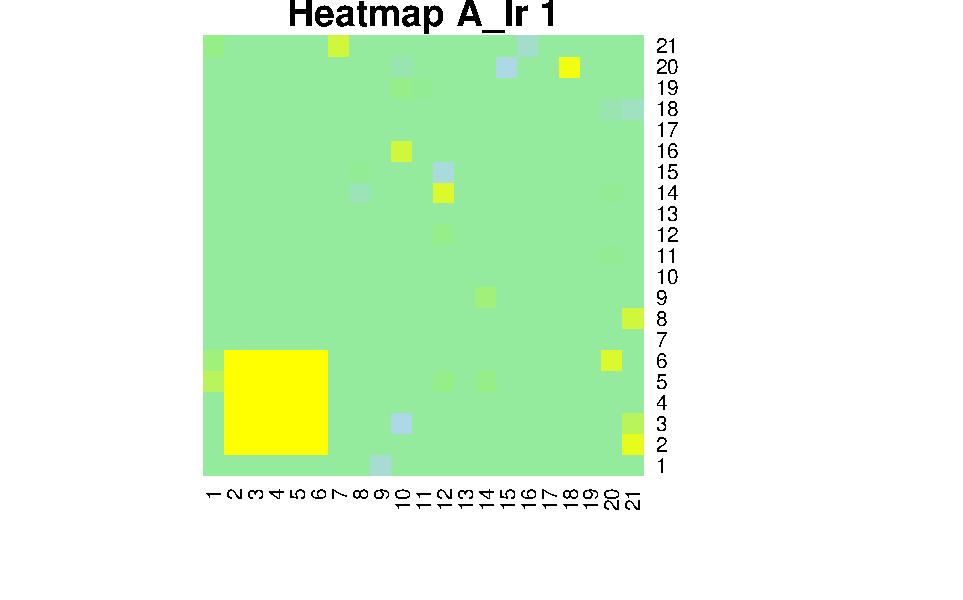
\includegraphics[width=.25\linewidth]{plots/alr1.pdf}
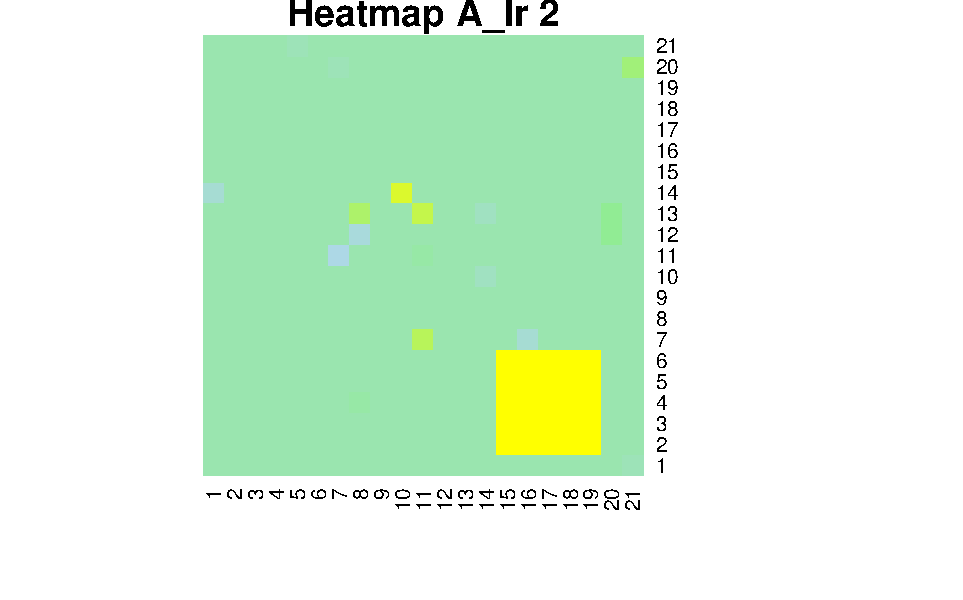
\includegraphics[width=.25\linewidth]{plots/alr2.pdf}\\
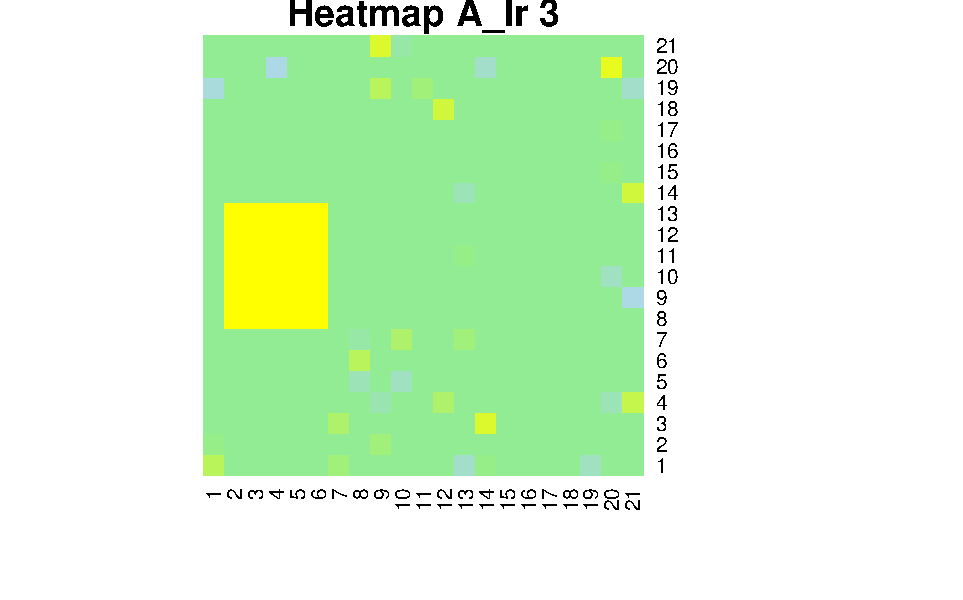
\includegraphics[width=.25\linewidth]{plots/alr3.pdf}
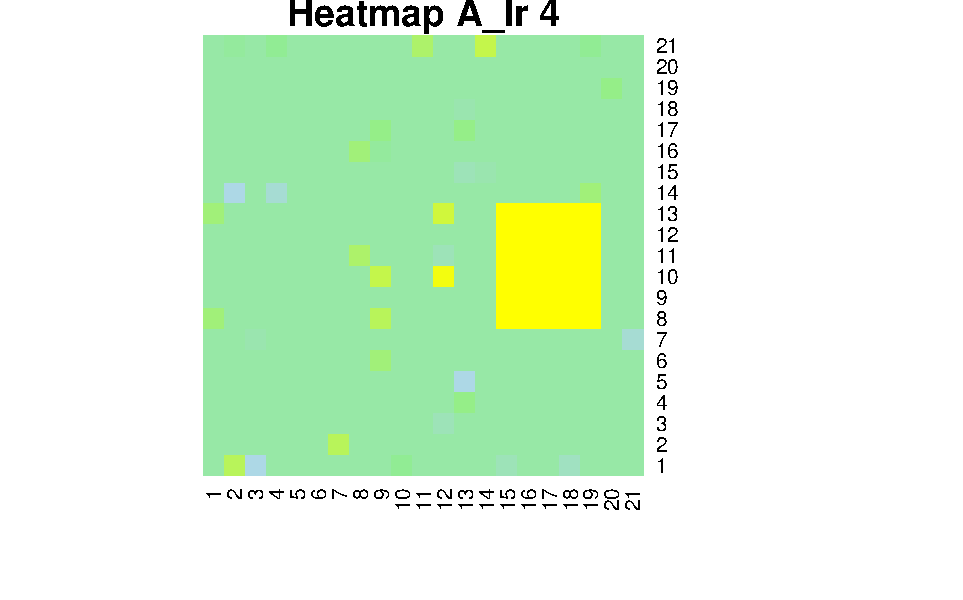
\includegraphics[width=.25\linewidth]{plots/alr4.pdf}
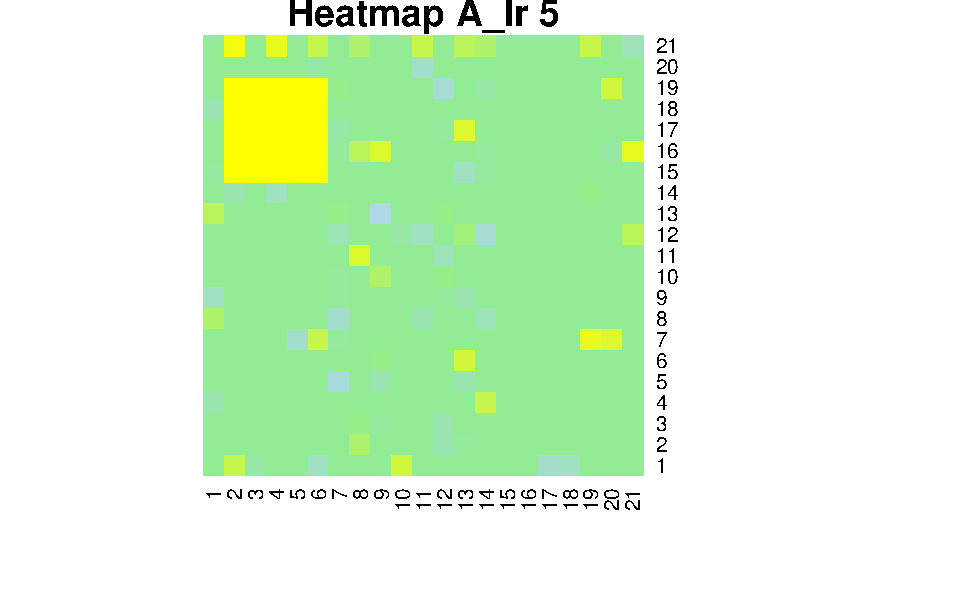
\includegraphics[width=.25\linewidth]{plots/alr5.pdf}
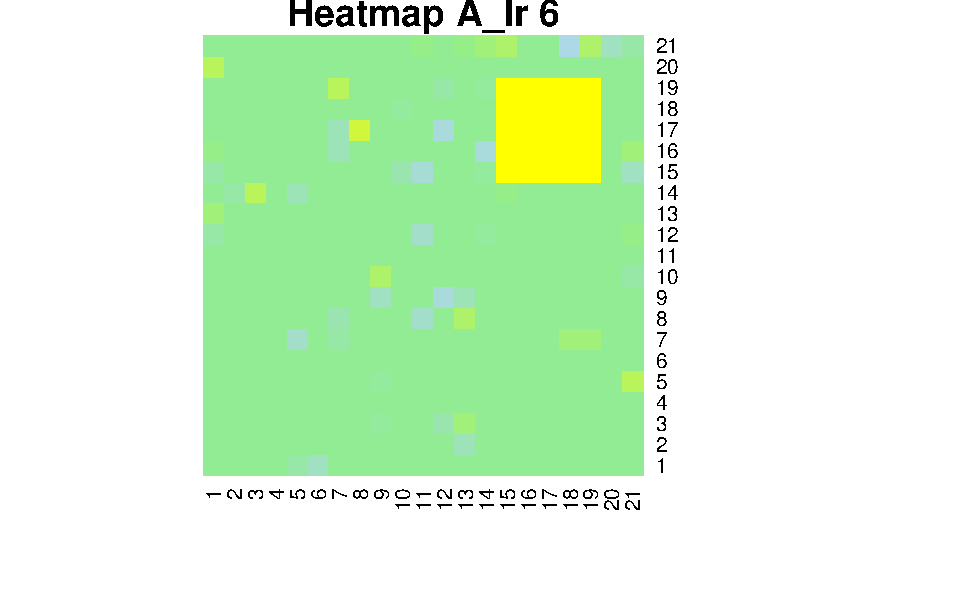
\includegraphics[width=.25\linewidth]{plots/alr6.pdf}\\\\
$\textbf{D}_{rr}$ and $\textbf{D}_{lr}$ are graphed respectively below.\\
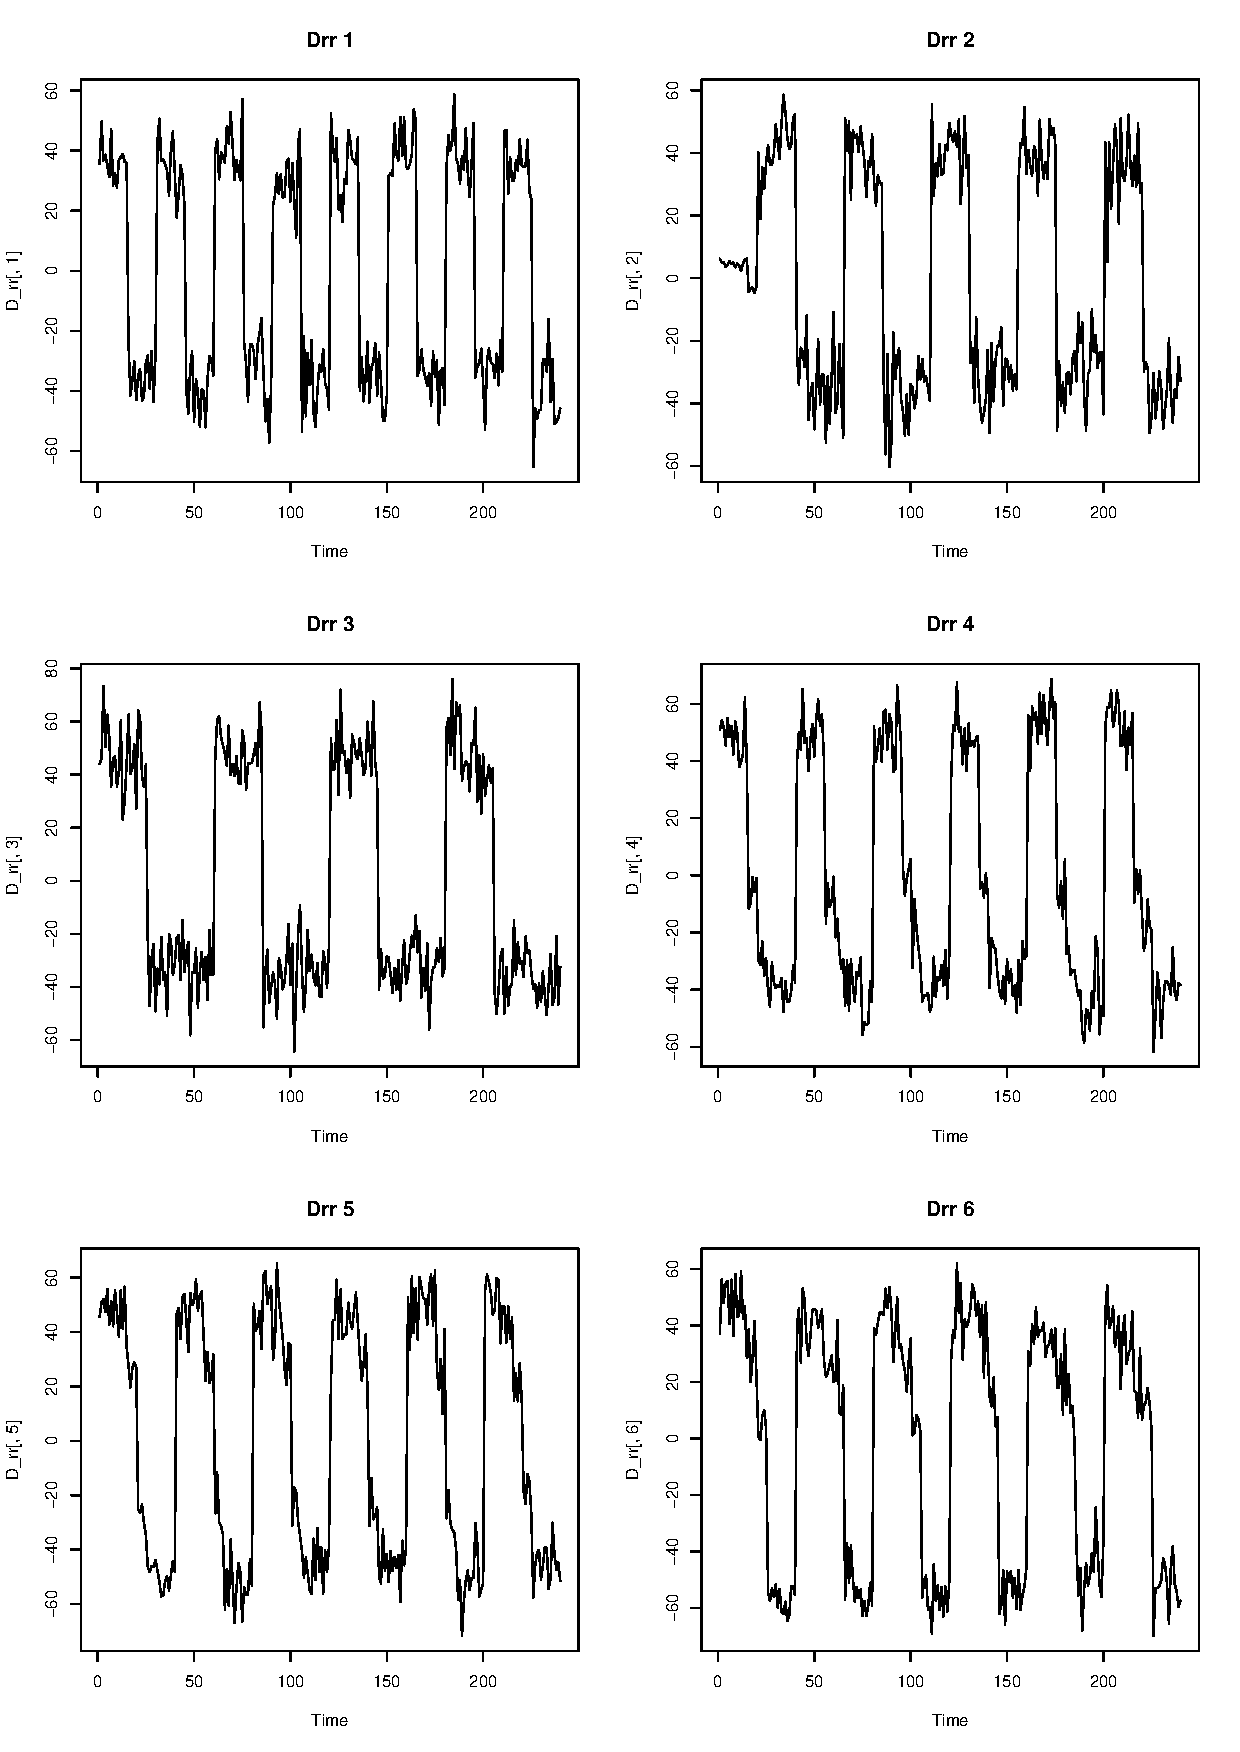
\includegraphics[width=.55\linewidth]{plots/better_drr_subplots.pdf}
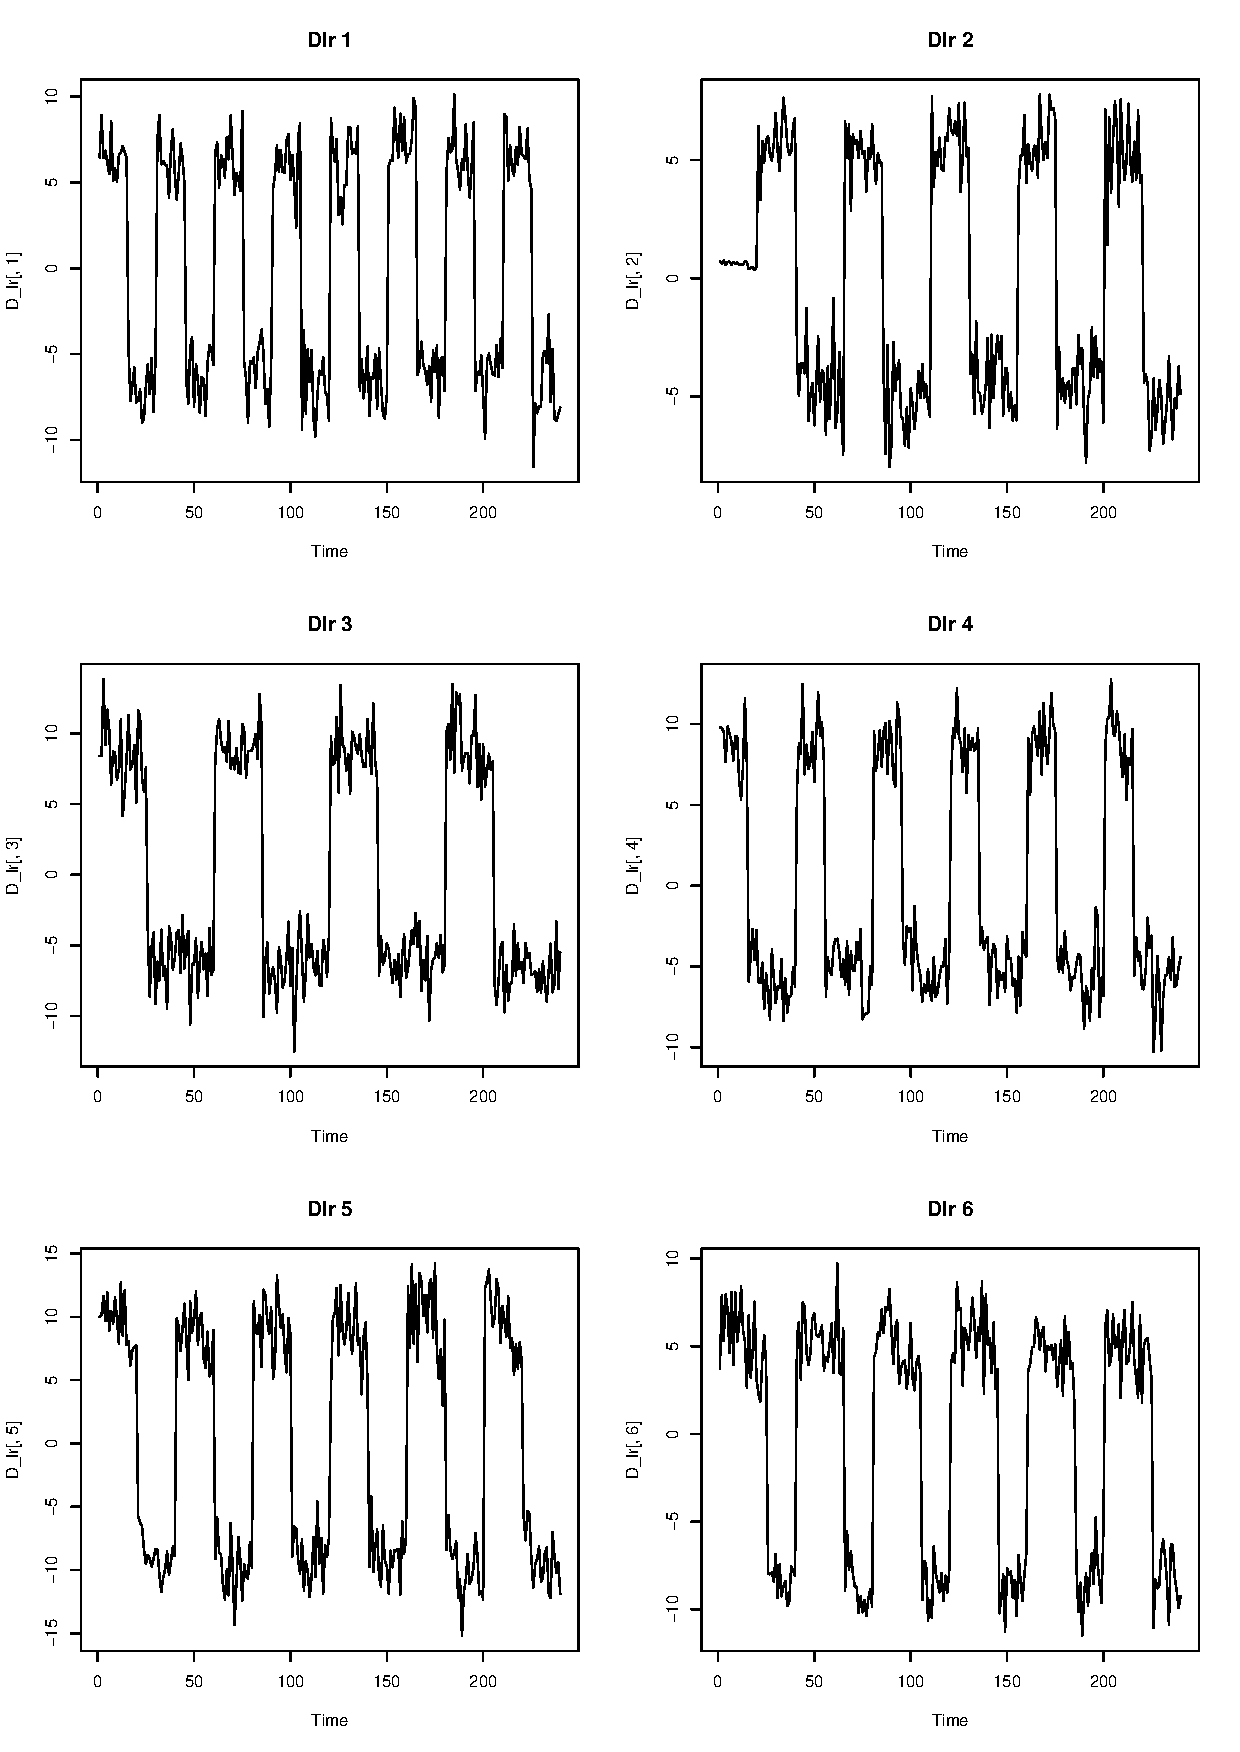
\includegraphics[width=.55\linewidth]{plots/dlr_subplots.pdf}\\
The reason behind the difference in the estimates of $\textbf{A}$ is that LR has an optimised regularization term, $\rho$, which penalises the $l-1$ norm used to estimate $\textbf{A}$.\\\\
\textbf{2.5}\\
Below are plots of the eigen values of the PCs. The first graph contains all 6 TCs' eigen values, and then they are plotted individually.\\
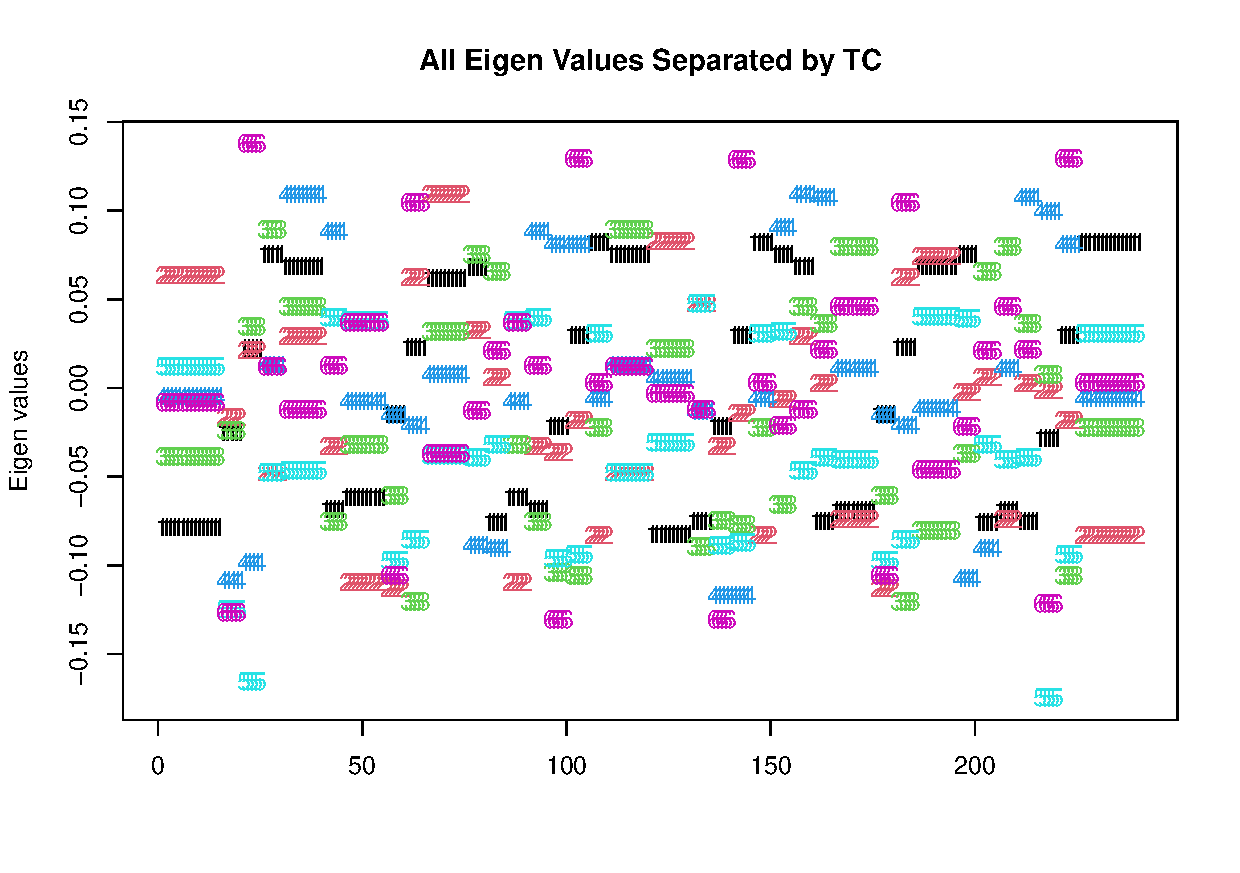
\includegraphics[width=.75\linewidth]{plots/ALL_eigen_values.pdf}\\
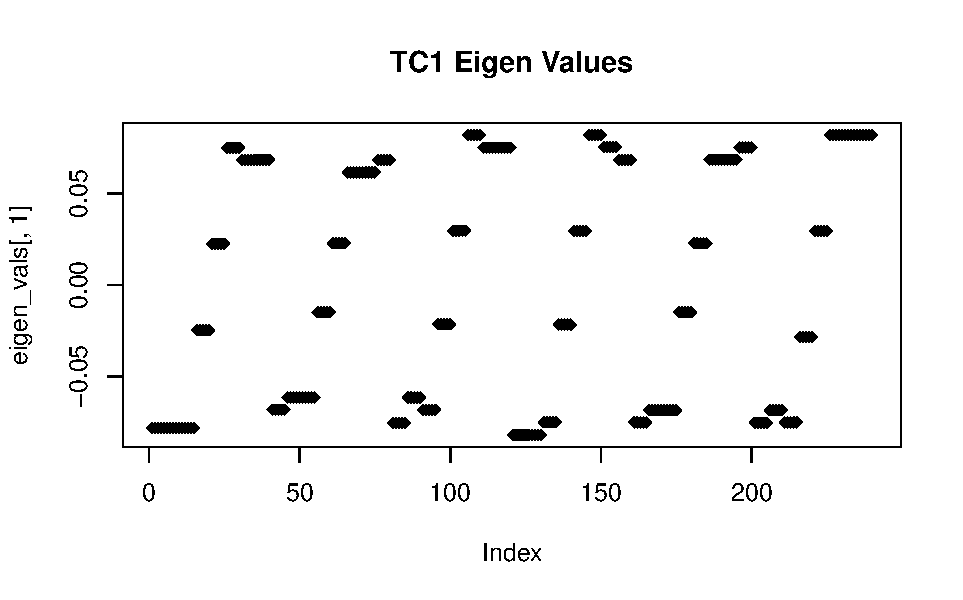
\includegraphics[width=.35\linewidth]{plots/tc1_eigen.pdf}
\includegraphics[width=.35\linewidth]{plots/tc2_eigen.pdf}
\includegraphics[width=.35\linewidth]{plots/tc3_eigen.pdf}\\
\includegraphics[width=.35\linewidth]{plots/tc4_eigen.pdf}
\includegraphics[width=.35\linewidth]{plots/tc5_eigen.pdf}
\includegraphics[width=.35\linewidth]{plots/tc6_eigen.pdf}\\
The fifth PC has the smallest eigen values.\\
\includegraphics[width=.65\linewidth]{plots/z_plots.pdf}
\includegraphics[width=.45\linewidth]{plots/1_1plots_3x2.pdf}\\
The deteriorated shape is due to the dimensionality reduction that is inherent to PCA.\\\\
Now after applying Lasso Regression on \textbf{Z}:\\
\includegraphics[width=.35\linewidth]{plots/apcr1.pdf}
\includegraphics[width=.35\linewidth]{plots/apcr2.pdf}
\includegraphics[width=.35\linewidth]{plots/apcr3.pdf}\\
\includegraphics[width=.35\linewidth]{plots/apcr4.pdf}
\includegraphics[width=.35\linewidth]{plots/apcr5.pdf}
\includegraphics[width=.35\linewidth]{plots/apcr6.pdf}\\

\includegraphics[width=.55\linewidth]{plots/Dpcr_subplots.pdf}\\\\
The PCR performed worse than the other three regression models largely to its focus on dimensionality reduction, which in the case of this dataset is not needed or used. Hence when performing PCR here, not much benefit is gained as we are not utilising the primary reason to use PCA, and hence it is distorting the shape of the TCs.
\end{document}
